\documentclass[1p]{elsarticle_modified}
%\bibliographystyle{elsarticle-num}

%\usepackage[colorlinks]{hyperref}
%\usepackage{abbrmath_seonhwa} %\Abb, \Ascr, \Acal ,\Abf, \Afrak
\usepackage{amsfonts}
\usepackage{amssymb}
\usepackage{amsmath}
\usepackage{amsthm}
\usepackage{scalefnt}
\usepackage{amsbsy}
\usepackage{kotex}
\usepackage{caption}
\usepackage{subfig}
\usepackage{color}
\usepackage{graphicx}
\usepackage{xcolor} %% white, black, red, green, blue, cyan, magenta, yellow
\usepackage{float}
\usepackage{setspace}
\usepackage{hyperref}

\usepackage{tikz}
\usetikzlibrary{arrows}

\usepackage{multirow}
\usepackage{array} % fixed length table
\usepackage{hhline}

%%%%%%%%%%%%%%%%%%%%%
\makeatletter
\renewcommand*\env@matrix[1][\arraystretch]{%
	\edef\arraystretch{#1}%
	\hskip -\arraycolsep
	\let\@ifnextchar\new@ifnextchar
	\array{*\c@MaxMatrixCols c}}
\makeatother %https://tex.stackexchange.com/questions/14071/how-can-i-increase-the-line-spacing-in-a-matrix
%%%%%%%%%%%%%%%

\usepackage[normalem]{ulem}

\newcommand{\msout}[1]{\ifmmode\text{\sout{\ensuremath{#1}}}\else\sout{#1}\fi}
%SOURCE: \msout is \stkout macro in https://tex.stackexchange.com/questions/20609/strikeout-in-math-mode

\newcommand{\cancel}[1]{
	\ifmmode
	{\color{red}\msout{#1}}
	\else
	{\color{red}\sout{#1}}
	\fi
}

\newcommand{\add}[1]{
	{\color{blue}\uwave{#1}}
}

\newcommand{\replace}[2]{
	\ifmmode
	{\color{red}\msout{#1}}{\color{blue}\uwave{#2}}
	\else
	{\color{red}\sout{#1}}{\color{blue}\uwave{#2}}
	\fi
}

\newcommand{\Sol}{\mathcal{S}} %segment
\newcommand{\D}{D} %diagram
\newcommand{\A}{\mathcal{A}} %arc


%%%%%%%%%%%%%%%%%%%%%%%%%%%%%5 test

\def\sl{\operatorname{\textup{SL}}(2,\Cbb)}
\def\psl{\operatorname{\textup{PSL}}(2,\Cbb)}
\def\quan{\mkern 1mu \triangleright \mkern 1mu}

\theoremstyle{definition}
\newtheorem{thm}{Theorem}[section]
\newtheorem{prop}[thm]{Proposition}
\newtheorem{lem}[thm]{Lemma}
\newtheorem{ques}[thm]{Question}
\newtheorem{cor}[thm]{Corollary}
\newtheorem{defn}[thm]{Definition}
\newtheorem{exam}[thm]{Example}
\newtheorem{rmk}[thm]{Remark}
\newtheorem{alg}[thm]{Algorithm}

\newcommand{\I}{\sqrt{-1}}
\begin{document}

%\begin{frontmatter}
%
%\title{Boundary parabolic representations of knots up to 8 crossings}
%
%%% Group authors per affiliation:
%\author{Yunhi Cho} 
%\address{Department of Mathematics, University of Seoul, Seoul, Korea}
%\ead{yhcho@uos.ac.kr}
%
%
%\author{Seonhwa Kim} %\fnref{s_kim}}
%\address{Center for Geometry and Physics, Institute for Basic Science, Pohang, 37673, Korea}
%\ead{ryeona17@ibs.re.kr}
%
%\author{Hyuk Kim}
%\address{Department of Mathematical Sciences, Seoul National University, Seoul 08826, Korea}
%\ead{hyukkim@snu.ac.kr}
%
%\author{Seokbeom Yoon}
%\address{Department of Mathematical Sciences, Seoul National University, Seoul, 08826,  Korea}
%\ead{sbyoon15@snu.ac.kr}
%
%\begin{abstract}
%We find all boundary parabolic representation of knots up to 8 crossings.
%
%\end{abstract}
%\begin{keyword}
%    \MSC[2010] 57M25 
%\end{keyword}
%
%\end{frontmatter}

%\linenumbers
%\tableofcontents
%
\newcommand\colored[1]{\textcolor{white}{\rule[-0.35ex]{0.8em}{1.4ex}}\kern-0.8em\color{red} #1}%
%\newcommand\colored[1]{\textcolor{white}{ #1}\kern-2.17ex	\textcolor{white}{ #1}\kern-1.81ex	\textcolor{white}{ #1}\kern-2.15ex\color{red}#1	}

{\Large $\underline{12a_{1057}~(K12a_{1057})}$}

\setlength{\tabcolsep}{10pt}
\renewcommand{\arraystretch}{1.6}
\vspace{1cm}\begin{tabular}{m{100pt}>{\centering\arraybackslash}m{274pt}}
\multirow{5}{120pt}{
	\centering
	\includegraphics[width=112pt]{../../../GIT/diagram.site/Diagrams/png/1858_12a_1057.png}\\
\ \ \ A knot diagram\footnotemark}&
\allowdisplaybreaks
\textbf{Linearized knot diagam} \\
\cline{2-2}
 &
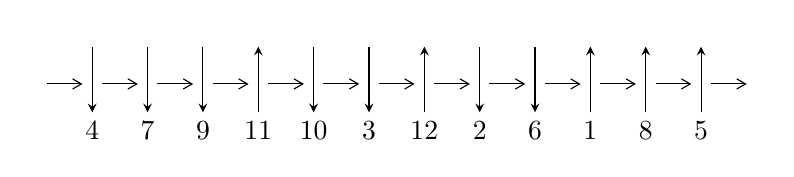
\begin{tikzpicture}[x=20pt, y=17pt]
	% nodes
	\node (C0) at (0, 0) {};
	\node (C1) at (1, 0) {};
	\node (C1U) at (1, +1) {};
	\node (C1D) at (1, -1) {4};

	\node (C2) at (2, 0) {};
	\node (C2U) at (2, +1) {};
	\node (C2D) at (2, -1) {7};

	\node (C3) at (3, 0) {};
	\node (C3U) at (3, +1) {};
	\node (C3D) at (3, -1) {9};

	\node (C4) at (4, 0) {};
	\node (C4U) at (4, +1) {};
	\node (C4D) at (4, -1) {11};

	\node (C5) at (5, 0) {};
	\node (C5U) at (5, +1) {};
	\node (C5D) at (5, -1) {10};

	\node (C6) at (6, 0) {};
	\node (C6U) at (6, +1) {};
	\node (C6D) at (6, -1) {3};

	\node (C7) at (7, 0) {};
	\node (C7U) at (7, +1) {};
	\node (C7D) at (7, -1) {12};

	\node (C8) at (8, 0) {};
	\node (C8U) at (8, +1) {};
	\node (C8D) at (8, -1) {2};

	\node (C9) at (9, 0) {};
	\node (C9U) at (9, +1) {};
	\node (C9D) at (9, -1) {6};

	\node (C10) at (10, 0) {};
	\node (C10U) at (10, +1) {};
	\node (C10D) at (10, -1) {1};

	\node (C11) at (11, 0) {};
	\node (C11U) at (11, +1) {};
	\node (C11D) at (11, -1) {8};

	\node (C12) at (12, 0) {};
	\node (C12U) at (12, +1) {};
	\node (C12D) at (12, -1) {5};
	\node (C13) at (13, 0) {};

	% arrows
	\draw[->,>={angle 60}]
	(C0) edge (C1) (C1) edge (C2) (C2) edge (C3) (C3) edge (C4) (C4) edge (C5) (C5) edge (C6) (C6) edge (C7) (C7) edge (C8) (C8) edge (C9) (C9) edge (C10) (C10) edge (C11) (C11) edge (C12) (C12) edge (C13) ;	\draw[->,>=stealth]
	(C1U) edge (C1D) (C2U) edge (C2D) (C3U) edge (C3D) (C4D) edge (C4U) (C5U) edge (C5D) (C6U) edge (C6D) (C7D) edge (C7U) (C8U) edge (C8D) (C9U) edge (C9D) (C10D) edge (C10U) (C11D) edge (C11U) (C12D) edge (C12U) ;
	\end{tikzpicture} \\
\hhline{~~} \\& 
\textbf{Solving Sequence} \\ \cline{2-2} 
 &
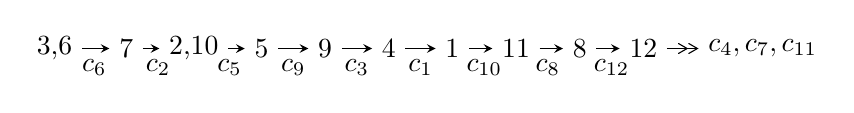
\begin{tikzpicture}[x=23pt, y=7pt]
	% node
	\node (A0) at (-1/8, 0) {3,6};
	\node (A1) at (1, 0) {7};
	\node (A2) at (33/16, 0) {2,10};
	\node (A3) at (25/8, 0) {5};
	\node (A4) at (33/8, 0) {9};
	\node (A5) at (41/8, 0) {4};
	\node (A6) at (49/8, 0) {1};
	\node (A7) at (57/8, 0) {11};
	\node (A8) at (65/8, 0) {8};
	\node (A9) at (73/8, 0) {12};
	\node (C1) at (1/2, -1) {$c_{6}$};
	\node (C2) at (3/2, -1) {$c_{2}$};
	\node (C3) at (21/8, -1) {$c_{5}$};
	\node (C4) at (29/8, -1) {$c_{9}$};
	\node (C5) at (37/8, -1) {$c_{3}$};
	\node (C6) at (45/8, -1) {$c_{1}$};
	\node (C7) at (53/8, -1) {$c_{10}$};
	\node (C8) at (61/8, -1) {$c_{8}$};
	\node (C9) at (69/8, -1) {$c_{12}$};
	\node (A10) at (11, 0) {$c_{4},c_{7},c_{11}$};

	% edge
	\draw[->,>=stealth]	
	(A0) edge (A1) (A1) edge (A2) (A2) edge (A3) (A3) edge (A4) (A4) edge (A5) (A5) edge (A6) (A6) edge (A7) (A7) edge (A8) (A8) edge (A9) ;
	\draw[->>,>={angle 60}]	
	(A9) edge (A10);
\end{tikzpicture} \\ 

\end{tabular} \\

\footnotetext{
The image of knot diagram is generated by the software ``\textbf{Draw programme}" developed by Andrew Bartholomew(\url{http://www.layer8.co.uk/maths/draw/index.htm\#Running-draw}), where we modified some parts for our purpose(\url{https://github.com/CATsTAILs/LinksPainter}).
}\phantom \\ \newline 
\centering \textbf{Ideals for irreducible components\footnotemark of $X_{\text{par}}$} 
 
\begin{align*}
I^u_{1}&=\langle 
1.95047\times10^{1094} u^{167}-5.59776\times10^{1093} u^{166}+\cdots+2.59133\times10^{1097} b-9.58013\times10^{1097},\\
\phantom{I^u_{1}}&\phantom{= \langle  }-5.16111\times10^{1098} u^{167}+3.11285\times10^{1097} u^{166}+\cdots+5.14353\times10^{1101} a+2.81343\times10^{1103},\\
\phantom{I^u_{1}}&\phantom{= \langle  }u^{168}- u^{167}+\cdots-545381 u+39698\rangle \\
I^u_{2}&=\langle 
7.30617\times10^{64} u^{43}-2.12038\times10^{65} u^{42}+\cdots+1.06566\times10^{66} b-1.02238\times10^{66},\\
\phantom{I^u_{2}}&\phantom{= \langle  }2.38557\times10^{66} u^{43}-1.01455\times10^{67} u^{42}+\cdots+2.02475\times10^{67} a-1.52864\times10^{68},\;u^{44}-2 u^{43}+\cdots+87 u+19\rangle \\
\\
\end{align*}
\raggedright * 2 irreducible components of $\dim_{\mathbb{C}}=0$, with total 212 representations.\\
\footnotetext{All coefficients of polynomials are rational numbers. But the coefficients are sometimes approximated in decimal forms when there is not enough margin.}
\newpage
\renewcommand{\arraystretch}{1}
\centering \section*{I. $I^u_{1}= \langle 1.95\times10^{1094} u^{167}-5.60\times10^{1093} u^{166}+\cdots+2.59\times10^{1097} b-9.58\times10^{1097},\;-5.16\times10^{1098} u^{167}+3.11\times10^{1097} u^{166}+\cdots+5.14\times10^{1101} a+2.81\times10^{1103},\;u^{168}- u^{167}+\cdots-545381 u+39698 \rangle$}
\flushleft \textbf{(i) Arc colorings}\\
\begin{tabular}{m{7pt} m{180pt} m{7pt} m{180pt} }
\flushright $a_{3}=$&$\begin{pmatrix}0\\u\end{pmatrix}$ \\
\flushright $a_{6}=$&$\begin{pmatrix}1\\0\end{pmatrix}$ \\
\flushright $a_{7}=$&$\begin{pmatrix}1\\u^2\end{pmatrix}$ \\
\flushright $a_{2}=$&$\begin{pmatrix}u\\u^3+u\end{pmatrix}$ \\
\flushright $a_{10}=$&$\begin{pmatrix}0.00100342 u^{167}-0.0000605198 u^{166}+\cdots+584.974 u-54.6984\\-0.000752692 u^{167}+0.000216019 u^{166}+\cdots-90.6208 u+3.69699\end{pmatrix}$ \\
\flushright $a_{5}=$&$\begin{pmatrix}0.000971291 u^{167}-0.0000747615 u^{166}+\cdots-442.583 u+25.6220\\-0.00114684 u^{167}+0.000993880 u^{166}+\cdots-397.386 u+36.3783\end{pmatrix}$ \\
\flushright $a_{9}=$&$\begin{pmatrix}0.000250724 u^{167}+0.000155499 u^{166}+\cdots+494.354 u-51.0014\\-0.000752692 u^{167}+0.000216019 u^{166}+\cdots-90.6208 u+3.69699\end{pmatrix}$ \\
\flushright $a_{4}=$&$\begin{pmatrix}-0.00531893 u^{167}+0.00730716 u^{166}+\cdots-1189.66 u+68.5404\\0.000743565 u^{167}-0.00101886 u^{166}+\cdots-33.7436 u+6.96915\end{pmatrix}$ \\
\flushright $a_{1}=$&$\begin{pmatrix}-0.00215895 u^{167}+0.000694507 u^{166}+\cdots+587.392 u-45.0724\\0.000209614 u^{167}+0.00108263 u^{166}+\cdots-407.374 u+26.4468\end{pmatrix}$ \\
\flushright $a_{11}=$&$\begin{pmatrix}0.00289672 u^{167}-0.000930766 u^{166}+\cdots+517.763 u-44.6072\\-0.000721998 u^{167}-0.000584795 u^{166}+\cdots+200.427 u-13.6036\end{pmatrix}$ \\
\flushright $a_{8}=$&$\begin{pmatrix}0.00118509 u^{167}+0.000227451 u^{166}+\cdots+202.289 u-26.0549\\-0.000852012 u^{167}-0.000278598 u^{166}+\cdots+129.051 u-11.3055\end{pmatrix}$ \\
\flushright $a_{12}=$&$\begin{pmatrix}-0.000339869 u^{167}-0.000484650 u^{166}+\cdots-386.806 u+28.9363\\0.000423902 u^{167}-0.0000378799 u^{166}+\cdots-9.01557 u+4.98085\end{pmatrix}$\\&\end{tabular}
\flushleft \textbf{(ii) Obstruction class $= -1$}\\~\\
\flushleft \textbf{(iii) Cusp Shapes $= 0.00776499 u^{167}-0.0212134 u^{166}+\cdots+8536.45 u-617.062$}\\~\\
\newpage\renewcommand{\arraystretch}{1}
\flushleft \textbf{(iv) u-Polynomials at the component}\newline \\
\begin{tabular}{m{50pt}|m{274pt}}
Crossings & \hspace{64pt}u-Polynomials at each crossing \\
\hline $$\begin{aligned}c_{1}\end{aligned}$$&$\begin{aligned}
&u^{168}-13 u^{167}+\cdots-21712189323 u+1419536343
\end{aligned}$\\
\hline $$\begin{aligned}c_{2},c_{6}\end{aligned}$$&$\begin{aligned}
&u^{168}- u^{167}+\cdots-545381 u+39698
\end{aligned}$\\
\hline $$\begin{aligned}c_{3}\end{aligned}$$&$\begin{aligned}
&u^{168}-2 u^{167}+\cdots-7408948459 u+395731121
\end{aligned}$\\
\hline $$\begin{aligned}c_{4}\end{aligned}$$&$\begin{aligned}
&u^{168}-6 u^{167}+\cdots+457 u+19
\end{aligned}$\\
\hline $$\begin{aligned}c_{5},c_{9}\end{aligned}$$&$\begin{aligned}
&u^{168}+77 u^{166}+\cdots-46998156 u+3044193
\end{aligned}$\\
\hline $$\begin{aligned}c_{7},c_{11}\end{aligned}$$&$\begin{aligned}
&u^{168}+44 u^{166}+\cdots-10323 u+2217
\end{aligned}$\\
\hline $$\begin{aligned}c_{8}\end{aligned}$$&$\begin{aligned}
&u^{168}-4 u^{167}+\cdots-7477336 u+3141661
\end{aligned}$\\
\hline $$\begin{aligned}c_{10}\end{aligned}$$&$\begin{aligned}
&u^{168}+12 u^{167}+\cdots+63876 u+5329
\end{aligned}$\\
\hline $$\begin{aligned}c_{12}\end{aligned}$$&$\begin{aligned}
&u^{168}-9 u^{167}+\cdots+2597039 u+180482
\end{aligned}$\\
\hline
\end{tabular}\\~\\
\newpage\renewcommand{\arraystretch}{1}
\flushleft \textbf{(v) Riley Polynomials at the component}\newline \\
\begin{tabular}{m{50pt}|m{274pt}}
Crossings & \hspace{64pt}Riley Polynomials at each crossing \\
\hline $$\begin{aligned}c_{1}\end{aligned}$$&$\begin{aligned}
&y^{168}+41 y^{167}+\cdots+9.35\times10^{19} y+2.02\times10^{18}
\end{aligned}$\\
\hline $$\begin{aligned}c_{2},c_{6}\end{aligned}$$&$\begin{aligned}
&y^{168}+121 y^{167}+\cdots+51727293639 y+1575931204
\end{aligned}$\\
\hline $$\begin{aligned}c_{3}\end{aligned}$$&$\begin{aligned}
&y^{168}+200 y^{167}+\cdots+1.07\times10^{18} y+1.57\times10^{17}
\end{aligned}$\\
\hline $$\begin{aligned}c_{4}\end{aligned}$$&$\begin{aligned}
&y^{168}-22 y^{167}+\cdots-12313 y+361
\end{aligned}$\\
\hline $$\begin{aligned}c_{5},c_{9}\end{aligned}$$&$\begin{aligned}
&y^{168}+154 y^{167}+\cdots-30381005547372 y+9267111021249
\end{aligned}$\\
\hline $$\begin{aligned}c_{7},c_{11}\end{aligned}$$&$\begin{aligned}
&y^{168}+88 y^{167}+\cdots+213632547 y+4915089
\end{aligned}$\\
\hline $$\begin{aligned}c_{8}\end{aligned}$$&$\begin{aligned}
&y^{168}+46 y^{167}+\cdots+3241576894776324 y+9870033838921
\end{aligned}$\\
\hline $$\begin{aligned}c_{10}\end{aligned}$$&$\begin{aligned}
&y^{168}-28 y^{167}+\cdots-789826932 y+28398241
\end{aligned}$\\
\hline $$\begin{aligned}c_{12}\end{aligned}$$&$\begin{aligned}
&y^{168}-67 y^{167}+\cdots-2984683484193 y+32573752324
\end{aligned}$\\
\hline
\end{tabular}\\~\\
\newpage\flushleft \textbf{(vi) Complex Volumes and Cusp Shapes}
$$\begin{array}{c|c|c}  
\text{Solutions to }I^u_{1}& \I (\text{vol} + \sqrt{-1}CS) & \text{Cusp shape}\\
 \hline 
\begin{aligned}
u &= \phantom{-}0.284091 + 0.940316 I \\
a &= \phantom{-}0.337258 + 0.002796 I \\
b &= \phantom{-}0.968174 - 0.100011 I\end{aligned}
 & -2.59253 - 4.98996 I & \phantom{-0.000000 } 0 \\ \hline\begin{aligned}
u &= \phantom{-}0.284091 - 0.940316 I \\
a &= \phantom{-}0.337258 - 0.002796 I \\
b &= \phantom{-}0.968174 + 0.100011 I\end{aligned}
 & -2.59253 + 4.98996 I & \phantom{-0.000000 } 0 \\ \hline\begin{aligned}
u &= -0.075135 + 1.021290 I \\
a &= -2.52222 + 0.42696 I \\
b &= -0.116441 + 0.433873 I\end{aligned}
 & \phantom{-}4.07468 + 0.22739 I & \phantom{-0.000000 } 0 \\ \hline\begin{aligned}
u &= -0.075135 - 1.021290 I \\
a &= -2.52222 - 0.42696 I \\
b &= -0.116441 - 0.433873 I\end{aligned}
 & \phantom{-}4.07468 - 0.22739 I & \phantom{-0.000000 } 0 \\ \hline\begin{aligned}
u &= \phantom{-}0.054287 + 1.029200 I \\
a &= \phantom{-}8.05437 - 3.33744 I \\
b &= -0.101327 + 1.023360 I\end{aligned}
 & \phantom{-}4.84108 + 0.37208 I & \phantom{-0.000000 } 0 \\ \hline\begin{aligned}
u &= \phantom{-}0.054287 - 1.029200 I \\
a &= \phantom{-}8.05437 + 3.33744 I \\
b &= -0.101327 - 1.023360 I\end{aligned}
 & \phantom{-}4.84108 - 0.37208 I & \phantom{-0.000000 } 0 \\ \hline\begin{aligned}
u &= \phantom{-}0.152995 + 0.954850 I \\
a &= -0.532906 + 0.070687 I \\
b &= \phantom{-}1.208750 + 0.414829 I\end{aligned}
 & \phantom{-}2.42868 - 2.38369 I & \phantom{-0.000000 } 0 \\ \hline\begin{aligned}
u &= \phantom{-}0.152995 - 0.954850 I \\
a &= -0.532906 - 0.070687 I \\
b &= \phantom{-}1.208750 - 0.414829 I\end{aligned}
 & \phantom{-}2.42868 + 2.38369 I & \phantom{-0.000000 } 0 \\ \hline\begin{aligned}
u &= \phantom{-}0.330430 + 0.888535 I \\
a &= -0.160363 + 0.542365 I \\
b &= \phantom{-}0.866964 - 0.576259 I\end{aligned}
 & -2.99366 + 1.12430 I & \phantom{-0.000000 } 0 \\ \hline\begin{aligned}
u &= \phantom{-}0.330430 - 0.888535 I \\
a &= -0.160363 - 0.542365 I \\
b &= \phantom{-}0.866964 + 0.576259 I\end{aligned}
 & -2.99366 - 1.12430 I & \phantom{-0.000000 } 0\\
 \hline 
 \end{array}$$\newpage$$\begin{array}{c|c|c}  
\text{Solutions to }I^u_{1}& \I (\text{vol} + \sqrt{-1}CS) & \text{Cusp shape}\\
 \hline 
\begin{aligned}
u &= \phantom{-}0.872420 + 0.347617 I \\
a &= -1.016720 + 0.628518 I \\
b &= -0.012132 - 1.184250 I\end{aligned}
 & \phantom{-}1.56919 - 5.09213 I & \phantom{-0.000000 } 0 \\ \hline\begin{aligned}
u &= \phantom{-}0.872420 - 0.347617 I \\
a &= -1.016720 - 0.628518 I \\
b &= -0.012132 + 1.184250 I\end{aligned}
 & \phantom{-}1.56919 + 5.09213 I & \phantom{-0.000000 } 0 \\ \hline\begin{aligned}
u &= \phantom{-}0.916579 + 0.155382 I \\
a &= \phantom{-}0.207841 + 0.760860 I \\
b &= -1.017910 + 0.165439 I\end{aligned}
 & -1.58389 + 9.27209 I & \phantom{-0.000000 } 0 \\ \hline\begin{aligned}
u &= \phantom{-}0.916579 - 0.155382 I \\
a &= \phantom{-}0.207841 - 0.760860 I \\
b &= -1.017910 - 0.165439 I\end{aligned}
 & -1.58389 - 9.27209 I & \phantom{-0.000000 } 0 \\ \hline\begin{aligned}
u &= -1.068940 + 0.074303 I \\
a &= \phantom{-}0.295966 + 0.461058 I \\
b &= \phantom{-}0.26471 - 1.41552 I\end{aligned}
 & \phantom{-}6.14787 + 8.11153 I & \phantom{-0.000000 } 0 \\ \hline\begin{aligned}
u &= -1.068940 - 0.074303 I \\
a &= \phantom{-}0.295966 - 0.461058 I \\
b &= \phantom{-}0.26471 + 1.41552 I\end{aligned}
 & \phantom{-}6.14787 - 8.11153 I & \phantom{-0.000000 } 0 \\ \hline\begin{aligned}
u &= -0.687326 + 0.620253 I \\
a &= -0.348519 - 0.778136 I \\
b &= -0.377798 + 0.175034 I\end{aligned}
 & -1.97033 + 4.36241 I & \phantom{-0.000000 } 0 \\ \hline\begin{aligned}
u &= -0.687326 - 0.620253 I \\
a &= -0.348519 + 0.778136 I \\
b &= -0.377798 - 0.175034 I\end{aligned}
 & -1.97033 - 4.36241 I & \phantom{-0.000000 } 0 \\ \hline\begin{aligned}
u &= -0.234753 + 1.079510 I \\
a &= -1.47923 + 0.07692 I \\
b &= \phantom{-}2.11071 + 0.12459 I\end{aligned}
 & \phantom{-}2.55592 + 2.82580 I & \phantom{-0.000000 } 0 \\ \hline\begin{aligned}
u &= -0.234753 - 1.079510 I \\
a &= -1.47923 - 0.07692 I \\
b &= \phantom{-}2.11071 - 0.12459 I\end{aligned}
 & \phantom{-}2.55592 - 2.82580 I & \phantom{-0.000000 } 0\\
 \hline 
 \end{array}$$\newpage$$\begin{array}{c|c|c}  
\text{Solutions to }I^u_{1}& \I (\text{vol} + \sqrt{-1}CS) & \text{Cusp shape}\\
 \hline 
\begin{aligned}
u &= \phantom{-}0.041621 + 1.122060 I \\
a &= \phantom{-}1.37919 - 3.51006 I \\
b &= \phantom{-}0.181163 + 1.243160 I\end{aligned}
 & \phantom{-}5.42114 - 1.40537 I & \phantom{-0.000000 } 0 \\ \hline\begin{aligned}
u &= \phantom{-}0.041621 - 1.122060 I \\
a &= \phantom{-}1.37919 + 3.51006 I \\
b &= \phantom{-}0.181163 - 1.243160 I\end{aligned}
 & \phantom{-}5.42114 + 1.40537 I & \phantom{-0.000000 } 0 \\ \hline\begin{aligned}
u &= -0.603325 + 0.615323 I \\
a &= \phantom{-}0.261334 + 0.297631 I \\
b &= \phantom{-}0.619144 - 0.184760 I\end{aligned}
 & -1.76726 + 0.42600 I & \phantom{-0.000000 } 0 \\ \hline\begin{aligned}
u &= -0.603325 - 0.615323 I \\
a &= \phantom{-}0.261334 - 0.297631 I \\
b &= \phantom{-}0.619144 + 0.184760 I\end{aligned}
 & -1.76726 - 0.42600 I & \phantom{-0.000000 } 0 \\ \hline\begin{aligned}
u &= -1.096960 + 0.307197 I \\
a &= \phantom{-}0.172374 + 0.007616 I \\
b &= -0.503733 - 0.553418 I\end{aligned}
 & -4.74008 + 1.00418 I & \phantom{-0.000000 } 0 \\ \hline\begin{aligned}
u &= -1.096960 - 0.307197 I \\
a &= \phantom{-}0.172374 - 0.007616 I \\
b &= -0.503733 + 0.553418 I\end{aligned}
 & -4.74008 - 1.00418 I & \phantom{-0.000000 } 0 \\ \hline\begin{aligned}
u &= \phantom{-}0.597290 + 0.617376 I \\
a &= -0.21314 + 1.83750 I \\
b &= -0.460376 - 0.816970 I\end{aligned}
 & -3.91577 - 4.73107 I & \phantom{-0.000000 } 0 \\ \hline\begin{aligned}
u &= \phantom{-}0.597290 - 0.617376 I \\
a &= -0.21314 - 1.83750 I \\
b &= -0.460376 + 0.816970 I\end{aligned}
 & -3.91577 + 4.73107 I & \phantom{-0.000000 } 0 \\ \hline\begin{aligned}
u &= -0.012233 + 1.146940 I \\
a &= \phantom{-}0.49221 - 2.24248 I \\
b &= -0.74527 + 1.38163 I\end{aligned}
 & \phantom{-}3.70584 + 1.52818 I & \phantom{-0.000000 } 0 \\ \hline\begin{aligned}
u &= -0.012233 - 1.146940 I \\
a &= \phantom{-}0.49221 + 2.24248 I \\
b &= -0.74527 - 1.38163 I\end{aligned}
 & \phantom{-}3.70584 - 1.52818 I & \phantom{-0.000000 } 0\\
 \hline 
 \end{array}$$\newpage$$\begin{array}{c|c|c}  
\text{Solutions to }I^u_{1}& \I (\text{vol} + \sqrt{-1}CS) & \text{Cusp shape}\\
 \hline 
\begin{aligned}
u &= \phantom{-}0.257184 + 1.119890 I \\
a &= -1.37631 + 1.42853 I \\
b &= -0.140027 - 1.371420 I\end{aligned}
 & \phantom{-}9.31262 - 1.14023 I & \phantom{-0.000000 } 0 \\ \hline\begin{aligned}
u &= \phantom{-}0.257184 - 1.119890 I \\
a &= -1.37631 - 1.42853 I \\
b &= -0.140027 + 1.371420 I\end{aligned}
 & \phantom{-}9.31262 + 1.14023 I & \phantom{-0.000000 } 0 \\ \hline\begin{aligned}
u &= \phantom{-}1.077880 + 0.414884 I \\
a &= \phantom{-}0.363476 - 0.810347 I \\
b &= \phantom{-}0.30692 + 1.52869 I\end{aligned}
 & \phantom{-}4.92777 - 1.44448 I & \phantom{-0.000000 } 0 \\ \hline\begin{aligned}
u &= \phantom{-}1.077880 - 0.414884 I \\
a &= \phantom{-}0.363476 + 0.810347 I \\
b &= \phantom{-}0.30692 - 1.52869 I\end{aligned}
 & \phantom{-}4.92777 + 1.44448 I & \phantom{-0.000000 } 0 \\ \hline\begin{aligned}
u &= \phantom{-}1.079680 + 0.423739 I \\
a &= \phantom{-}0.056329 - 0.685349 I \\
b &= -0.037536 + 1.133930 I\end{aligned}
 & \phantom{-}0.64950 - 2.60034 I & \phantom{-0.000000 } 0 \\ \hline\begin{aligned}
u &= \phantom{-}1.079680 - 0.423739 I \\
a &= \phantom{-}0.056329 + 0.685349 I \\
b &= -0.037536 - 1.133930 I\end{aligned}
 & \phantom{-}0.64950 + 2.60034 I & \phantom{-0.000000 } 0 \\ \hline\begin{aligned}
u &= \phantom{-}0.325289 + 1.116410 I \\
a &= \phantom{-}0.913354 + 0.326190 I \\
b &= -0.251026 + 0.405995 I\end{aligned}
 & \phantom{-}3.59684 + 1.00091 I & \phantom{-0.000000 } 0 \\ \hline\begin{aligned}
u &= \phantom{-}0.325289 - 1.116410 I \\
a &= \phantom{-}0.913354 - 0.326190 I \\
b &= -0.251026 - 0.405995 I\end{aligned}
 & \phantom{-}3.59684 - 1.00091 I & \phantom{-0.000000 } 0 \\ \hline\begin{aligned}
u &= -1.068720 + 0.459817 I \\
a &= \phantom{-}0.220794 + 0.142059 I \\
b &= -0.116356 - 1.193400 I\end{aligned}
 & -0.93471 - 3.70656 I & \phantom{-0.000000 } 0 \\ \hline\begin{aligned}
u &= -1.068720 - 0.459817 I \\
a &= \phantom{-}0.220794 - 0.142059 I \\
b &= -0.116356 + 1.193400 I\end{aligned}
 & -0.93471 + 3.70656 I & \phantom{-0.000000 } 0\\
 \hline 
 \end{array}$$\newpage$$\begin{array}{c|c|c}  
\text{Solutions to }I^u_{1}& \I (\text{vol} + \sqrt{-1}CS) & \text{Cusp shape}\\
 \hline 
\begin{aligned}
u &= -0.033393 + 0.832881 I \\
a &= \phantom{-}0.54437 - 3.66890 I \\
b &= -0.11135 + 3.31405 I\end{aligned}
 & \phantom{-}2.98518 - 1.88452 I & \phantom{-0.000000 } 0 \\ \hline\begin{aligned}
u &= -0.033393 - 0.832881 I \\
a &= \phantom{-}0.54437 + 3.66890 I \\
b &= -0.11135 - 3.31405 I\end{aligned}
 & \phantom{-}2.98518 + 1.88452 I & \phantom{-0.000000 } 0 \\ \hline\begin{aligned}
u &= \phantom{-}0.126950 + 1.163600 I \\
a &= \phantom{-}0.981919 + 0.242067 I \\
b &= -1.43108 - 0.48845 I\end{aligned}
 & \phantom{-}3.50059 + 1.53756 I & \phantom{-0.000000 } 0 \\ \hline\begin{aligned}
u &= \phantom{-}0.126950 - 1.163600 I \\
a &= \phantom{-}0.981919 - 0.242067 I \\
b &= -1.43108 + 0.48845 I\end{aligned}
 & \phantom{-}3.50059 - 1.53756 I & \phantom{-0.000000 } 0 \\ \hline\begin{aligned}
u &= \phantom{-}0.132565 + 1.165520 I \\
a &= \phantom{-}0.03915 + 2.53352 I \\
b &= \phantom{-}0.131501 - 1.357020 I\end{aligned}
 & \phantom{-}3.23214 - 4.63266 I & \phantom{-0.000000 } 0 \\ \hline\begin{aligned}
u &= \phantom{-}0.132565 - 1.165520 I \\
a &= \phantom{-}0.03915 - 2.53352 I \\
b &= \phantom{-}0.131501 + 1.357020 I\end{aligned}
 & \phantom{-}3.23214 + 4.63266 I & \phantom{-0.000000 } 0 \\ \hline\begin{aligned}
u &= \phantom{-}0.002666 + 1.178680 I \\
a &= \phantom{-}0.676809 - 1.175660 I \\
b &= -1.169270 + 0.646241 I\end{aligned}
 & \phantom{-}3.61163 + 1.55804 I & \phantom{-0.000000 } 0 \\ \hline\begin{aligned}
u &= \phantom{-}0.002666 - 1.178680 I \\
a &= \phantom{-}0.676809 + 1.175660 I \\
b &= -1.169270 - 0.646241 I\end{aligned}
 & \phantom{-}3.61163 - 1.55804 I & \phantom{-0.000000 } 0 \\ \hline\begin{aligned}
u &= -0.151285 + 1.177340 I \\
a &= \phantom{-}0.41329 + 2.07435 I \\
b &= \phantom{-}0.43226 - 1.75944 I\end{aligned}
 & \phantom{-}9.76091 + 5.72419 I & \phantom{-0.000000 } 0 \\ \hline\begin{aligned}
u &= -0.151285 - 1.177340 I \\
a &= \phantom{-}0.41329 - 2.07435 I \\
b &= \phantom{-}0.43226 + 1.75944 I\end{aligned}
 & \phantom{-}9.76091 - 5.72419 I & \phantom{-0.000000 } 0\\
 \hline 
 \end{array}$$\newpage$$\begin{array}{c|c|c}  
\text{Solutions to }I^u_{1}& \I (\text{vol} + \sqrt{-1}CS) & \text{Cusp shape}\\
 \hline 
\begin{aligned}
u &= \phantom{-}1.191460 + 0.012419 I \\
a &= \phantom{-}0.130565 - 0.489369 I \\
b &= -0.48860 + 1.38167 I\end{aligned}
 & \phantom{-}4.17351 + 5.38540 I & \phantom{-0.000000 } 0 \\ \hline\begin{aligned}
u &= \phantom{-}1.191460 - 0.012419 I \\
a &= \phantom{-}0.130565 + 0.489369 I \\
b &= -0.48860 - 1.38167 I\end{aligned}
 & \phantom{-}4.17351 - 5.38540 I & \phantom{-0.000000 } 0 \\ \hline\begin{aligned}
u &= \phantom{-}0.106663 + 1.188350 I \\
a &= \phantom{-}0.74450 + 3.33756 I \\
b &= -0.209570 - 1.299310 I\end{aligned}
 & \phantom{-}5.36863 - 10.42050 I & \phantom{-0.000000 } 0 \\ \hline\begin{aligned}
u &= \phantom{-}0.106663 - 1.188350 I \\
a &= \phantom{-}0.74450 - 3.33756 I \\
b &= -0.209570 + 1.299310 I\end{aligned}
 & \phantom{-}5.36863 + 10.42050 I & \phantom{-0.000000 } 0 \\ \hline\begin{aligned}
u &= \phantom{-}0.281264 + 1.164210 I \\
a &= -0.499617 - 0.363828 I \\
b &= -0.513387 + 0.105594 I\end{aligned}
 & \phantom{-}4.64422 - 1.12038 I & \phantom{-0.000000 } 0 \\ \hline\begin{aligned}
u &= \phantom{-}0.281264 - 1.164210 I \\
a &= -0.499617 + 0.363828 I \\
b &= -0.513387 - 0.105594 I\end{aligned}
 & \phantom{-}4.64422 + 1.12038 I & \phantom{-0.000000 } 0 \\ \hline\begin{aligned}
u &= -0.037426 + 1.206240 I \\
a &= \phantom{-}0.79761 - 1.93796 I \\
b &= \phantom{-}0.30922 + 1.42884 I\end{aligned}
 & \phantom{-}6.72614 + 3.11920 I & \phantom{-0.000000 } 0 \\ \hline\begin{aligned}
u &= -0.037426 - 1.206240 I \\
a &= \phantom{-}0.79761 + 1.93796 I \\
b &= \phantom{-}0.30922 - 1.42884 I\end{aligned}
 & \phantom{-}6.72614 - 3.11920 I & \phantom{-0.000000 } 0 \\ \hline\begin{aligned}
u &= \phantom{-}0.768231 + 0.179991 I \\
a &= -0.229004 + 1.107430 I \\
b &= -0.284457 - 0.213294 I\end{aligned}
 & -1.35961 + 3.34267 I & \phantom{-0.000000 } 0 \\ \hline\begin{aligned}
u &= \phantom{-}0.768231 - 0.179991 I \\
a &= -0.229004 - 1.107430 I \\
b &= -0.284457 + 0.213294 I\end{aligned}
 & -1.35961 - 3.34267 I & \phantom{-0.000000 } 0\\
 \hline 
 \end{array}$$\newpage$$\begin{array}{c|c|c}  
\text{Solutions to }I^u_{1}& \I (\text{vol} + \sqrt{-1}CS) & \text{Cusp shape}\\
 \hline 
\begin{aligned}
u &= -0.450237 + 1.129640 I \\
a &= \phantom{-}1.08159 - 0.92564 I \\
b &= -0.510383 - 0.205515 I\end{aligned}
 & \phantom{-}1.72094 + 7.82381 I & \phantom{-0.000000 } 0 \\ \hline\begin{aligned}
u &= -0.450237 - 1.129640 I \\
a &= \phantom{-}1.08159 + 0.92564 I \\
b &= -0.510383 + 0.205515 I\end{aligned}
 & \phantom{-}1.72094 - 7.82381 I & \phantom{-0.000000 } 0 \\ \hline\begin{aligned}
u &= -0.223436 + 1.196850 I \\
a &= \phantom{-}0.66162 + 1.75649 I \\
b &= \phantom{-}0.13681 - 1.56788 I\end{aligned}
 & \phantom{-}9.43294 - 3.08893 I & \phantom{-0.000000 } 0 \\ \hline\begin{aligned}
u &= -0.223436 - 1.196850 I \\
a &= \phantom{-}0.66162 - 1.75649 I \\
b &= \phantom{-}0.13681 + 1.56788 I\end{aligned}
 & \phantom{-}9.43294 + 3.08893 I & \phantom{-0.000000 } 0 \\ \hline\begin{aligned}
u &= -0.603518 + 1.059190 I \\
a &= \phantom{-}1.037450 + 0.799838 I \\
b &= \phantom{-}0.365907 - 1.270220 I\end{aligned}
 & \phantom{-}1.06458 + 9.62248 I & \phantom{-0.000000 } 0 \\ \hline\begin{aligned}
u &= -0.603518 - 1.059190 I \\
a &= \phantom{-}1.037450 - 0.799838 I \\
b &= \phantom{-}0.365907 + 1.270220 I\end{aligned}
 & \phantom{-}1.06458 - 9.62248 I & \phantom{-0.000000 } 0 \\ \hline\begin{aligned}
u &= -0.288687 + 1.184920 I \\
a &= \phantom{-}0.138652 - 0.314545 I \\
b &= -0.640046 + 0.202767 I\end{aligned}
 & \phantom{-}1.91202 + 2.76204 I & \phantom{-0.000000 } 0 \\ \hline\begin{aligned}
u &= -0.288687 - 1.184920 I \\
a &= \phantom{-}0.138652 + 0.314545 I \\
b &= -0.640046 - 0.202767 I\end{aligned}
 & \phantom{-}1.91202 - 2.76204 I & \phantom{-0.000000 } 0 \\ \hline\begin{aligned}
u &= -0.729160 + 0.251539 I \\
a &= \phantom{-}0.113384 + 0.359445 I \\
b &= -0.162744 + 1.309360 I\end{aligned}
 & \phantom{-}5.98268 + 2.64378 I & \phantom{-0.000000 } 0 \\ \hline\begin{aligned}
u &= -0.729160 - 0.251539 I \\
a &= \phantom{-}0.113384 - 0.359445 I \\
b &= -0.162744 - 1.309360 I\end{aligned}
 & \phantom{-}5.98268 - 2.64378 I & \phantom{-0.000000 } 0\\
 \hline 
 \end{array}$$\newpage$$\begin{array}{c|c|c}  
\text{Solutions to }I^u_{1}& \I (\text{vol} + \sqrt{-1}CS) & \text{Cusp shape}\\
 \hline 
\begin{aligned}
u &= \phantom{-}0.480899 + 0.602446 I \\
a &= \phantom{-}0.25722 + 1.91127 I \\
b &= -0.398759 - 0.332342 I\end{aligned}
 & -3.64248 + 1.82200 I & \phantom{-0.000000 } 0 \\ \hline\begin{aligned}
u &= \phantom{-}0.480899 - 0.602446 I \\
a &= \phantom{-}0.25722 - 1.91127 I \\
b &= -0.398759 + 0.332342 I\end{aligned}
 & -3.64248 - 1.82200 I & \phantom{-0.000000 } 0 \\ \hline\begin{aligned}
u &= -0.167326 + 1.223240 I \\
a &= \phantom{-}1.43020 - 0.48536 I \\
b &= -1.99388 + 0.26584 I\end{aligned}
 & \phantom{-}3.08839 - 1.01266 I & \phantom{-0.000000 } 0 \\ \hline\begin{aligned}
u &= -0.167326 - 1.223240 I \\
a &= \phantom{-}1.43020 + 0.48536 I \\
b &= -1.99388 - 0.26584 I\end{aligned}
 & \phantom{-}3.08839 + 1.01266 I & \phantom{-0.000000 } 0 \\ \hline\begin{aligned}
u &= \phantom{-}0.613271 + 0.457217 I \\
a &= \phantom{-}1.20656 - 0.91303 I \\
b &= \phantom{-}0.02728 + 1.44953 I\end{aligned}
 & \phantom{-}4.18721 - 2.06146 I & \phantom{-0.000000 } 0 \\ \hline\begin{aligned}
u &= \phantom{-}0.613271 - 0.457217 I \\
a &= \phantom{-}1.20656 + 0.91303 I \\
b &= \phantom{-}0.02728 - 1.44953 I\end{aligned}
 & \phantom{-}4.18721 + 2.06146 I & \phantom{-0.000000 } 0 \\ \hline\begin{aligned}
u &= -0.506691 + 1.148720 I \\
a &= \phantom{-}0.316184 + 1.041090 I \\
b &= \phantom{-}0.735259 - 0.880646 I\end{aligned}
 & -2.00361 + 4.47632 I & \phantom{-0.000000 } 0 \\ \hline\begin{aligned}
u &= -0.506691 - 1.148720 I \\
a &= \phantom{-}0.316184 - 1.041090 I \\
b &= \phantom{-}0.735259 + 0.880646 I\end{aligned}
 & -2.00361 - 4.47632 I & \phantom{-0.000000 } 0 \\ \hline\begin{aligned}
u &= \phantom{-}0.589422 + 1.110200 I \\
a &= \phantom{-}0.86112 - 1.60289 I \\
b &= \phantom{-}0.234834 + 1.376290 I\end{aligned}
 & \phantom{-}3.20575 - 3.50616 I & \phantom{-0.000000 } 0 \\ \hline\begin{aligned}
u &= \phantom{-}0.589422 - 1.110200 I \\
a &= \phantom{-}0.86112 + 1.60289 I \\
b &= \phantom{-}0.234834 - 1.376290 I\end{aligned}
 & \phantom{-}3.20575 + 3.50616 I & \phantom{-0.000000 } 0\\
 \hline 
 \end{array}$$\newpage$$\begin{array}{c|c|c}  
\text{Solutions to }I^u_{1}& \I (\text{vol} + \sqrt{-1}CS) & \text{Cusp shape}\\
 \hline 
\begin{aligned}
u &= \phantom{-}0.331843 + 1.229400 I \\
a &= \phantom{-}0.132358 + 0.910865 I \\
b &= -1.088970 - 0.554810 I\end{aligned}
 & \phantom{-}4.20739 - 8.28834 I & \phantom{-0.000000 } 0 \\ \hline\begin{aligned}
u &= \phantom{-}0.331843 - 1.229400 I \\
a &= \phantom{-}0.132358 - 0.910865 I \\
b &= -1.088970 + 0.554810 I\end{aligned}
 & \phantom{-}4.20739 + 8.28834 I & \phantom{-0.000000 } 0 \\ \hline\begin{aligned}
u &= -0.247895 + 1.286380 I \\
a &= \phantom{-}0.165331 + 0.102441 I \\
b &= \phantom{-}0.697266 + 0.124675 I\end{aligned}
 & \phantom{-}3.34055 + 6.58969 I & \phantom{-0.000000 } 0 \\ \hline\begin{aligned}
u &= -0.247895 - 1.286380 I \\
a &= \phantom{-}0.165331 - 0.102441 I \\
b &= \phantom{-}0.697266 - 0.124675 I\end{aligned}
 & \phantom{-}3.34055 - 6.58969 I & \phantom{-0.000000 } 0 \\ \hline\begin{aligned}
u &= \phantom{-}0.374340 + 1.259280 I \\
a &= -0.00127852 + 0.00998449 I \\
b &= \phantom{-}0.865450 + 0.053819 I\end{aligned}
 & \phantom{-}2.13115 - 7.55128 I & \phantom{-0.000000 } 0 \\ \hline\begin{aligned}
u &= \phantom{-}0.374340 - 1.259280 I \\
a &= -0.00127852 - 0.00998449 I \\
b &= \phantom{-}0.865450 - 0.053819 I\end{aligned}
 & \phantom{-}2.13115 + 7.55128 I & \phantom{-0.000000 } 0 \\ \hline\begin{aligned}
u &= \phantom{-}0.680355 + 0.026540 I \\
a &= \phantom{-}0.515047 + 0.436675 I \\
b &= \phantom{-}0.742057 + 0.409507 I\end{aligned}
 & \phantom{-}0.44173 - 4.57830 I & \phantom{-0.000000 } 0 \\ \hline\begin{aligned}
u &= \phantom{-}0.680355 - 0.026540 I \\
a &= \phantom{-}0.515047 - 0.436675 I \\
b &= \phantom{-}0.742057 - 0.409507 I\end{aligned}
 & \phantom{-}0.44173 + 4.57830 I & \phantom{-0.000000 } 0 \\ \hline\begin{aligned}
u &= \phantom{-}0.443186 + 1.246440 I \\
a &= -0.522997 - 0.802719 I \\
b &= \phantom{-}1.40031 + 0.55525 I\end{aligned}
 & \phantom{-}1.8632 - 14.1424 I & \phantom{-0.000000 } 0 \\ \hline\begin{aligned}
u &= \phantom{-}0.443186 - 1.246440 I \\
a &= -0.522997 + 0.802719 I \\
b &= \phantom{-}1.40031 - 0.55525 I\end{aligned}
 & \phantom{-}1.8632 + 14.1424 I & \phantom{-0.000000 } 0\\
 \hline 
 \end{array}$$\newpage$$\begin{array}{c|c|c}  
\text{Solutions to }I^u_{1}& \I (\text{vol} + \sqrt{-1}CS) & \text{Cusp shape}\\
 \hline 
\begin{aligned}
u &= -0.517897 + 0.405372 I \\
a &= \phantom{-}0.52244 - 1.72953 I \\
b &= -0.979303 + 0.352505 I\end{aligned}
 & \phantom{-}0.576668 + 0.247597 I & \phantom{-0.000000 } 0 \\ \hline\begin{aligned}
u &= -0.517897 - 0.405372 I \\
a &= \phantom{-}0.52244 + 1.72953 I \\
b &= -0.979303 - 0.352505 I\end{aligned}
 & \phantom{-}0.576668 - 0.247597 I & \phantom{-0.000000 } 0 \\ \hline\begin{aligned}
u &= -1.341690 + 0.123032 I \\
a &= -0.058656 - 0.685993 I \\
b &= -0.38668 + 1.41090 I\end{aligned}
 & \phantom{-}3.4615 + 14.1615 I & \phantom{-0.000000 } 0 \\ \hline\begin{aligned}
u &= -1.341690 - 0.123032 I \\
a &= -0.058656 + 0.685993 I \\
b &= -0.38668 - 1.41090 I\end{aligned}
 & \phantom{-}3.4615 - 14.1615 I & \phantom{-0.000000 } 0 \\ \hline\begin{aligned}
u &= \phantom{-}0.598970 + 0.235062 I \\
a &= \phantom{-}0.190700 - 0.931123 I \\
b &= \phantom{-}0.341182 + 0.958710 I\end{aligned}
 & \phantom{-}1.09668 - 2.85370 I & \phantom{-0.000000 } 0 \\ \hline\begin{aligned}
u &= \phantom{-}0.598970 - 0.235062 I \\
a &= \phantom{-}0.190700 + 0.931123 I \\
b &= \phantom{-}0.341182 - 0.958710 I\end{aligned}
 & \phantom{-}1.09668 + 2.85370 I & \phantom{-0.000000 } 0 \\ \hline\begin{aligned}
u &= -0.621178 + 0.158102 I \\
a &= \phantom{-}0.203826 - 0.770996 I \\
b &= \phantom{-}1.076030 - 0.176436 I\end{aligned}
 & -0.95765 - 3.74813 I & \phantom{-0.000000 } 0 \\ \hline\begin{aligned}
u &= -0.621178 - 0.158102 I \\
a &= \phantom{-}0.203826 + 0.770996 I \\
b &= \phantom{-}1.076030 + 0.176436 I\end{aligned}
 & -0.95765 + 3.74813 I & \phantom{-0.000000 } 0 \\ \hline\begin{aligned}
u &= \phantom{-}0.129231 + 1.356950 I \\
a &= -0.70488 + 1.47927 I \\
b &= -0.313586 - 1.205940 I\end{aligned}
 & \phantom{-}8.61587 - 1.20870 I & \phantom{-0.000000 } 0 \\ \hline\begin{aligned}
u &= \phantom{-}0.129231 - 1.356950 I \\
a &= -0.70488 - 1.47927 I \\
b &= -0.313586 + 1.205940 I\end{aligned}
 & \phantom{-}8.61587 + 1.20870 I & \phantom{-0.000000 } 0\\
 \hline 
 \end{array}$$\newpage$$\begin{array}{c|c|c}  
\text{Solutions to }I^u_{1}& \I (\text{vol} + \sqrt{-1}CS) & \text{Cusp shape}\\
 \hline 
\begin{aligned}
u &= -0.095784 + 1.395260 I \\
a &= -0.04280 - 1.96802 I \\
b &= -0.65687 + 1.67937 I\end{aligned}
 & \phantom{-}8.33970 + 9.96362 I & \phantom{-0.000000 } 0 \\ \hline\begin{aligned}
u &= -0.095784 - 1.395260 I \\
a &= -0.04280 + 1.96802 I \\
b &= -0.65687 - 1.67937 I\end{aligned}
 & \phantom{-}8.33970 - 9.96362 I & \phantom{-0.000000 } 0 \\ \hline\begin{aligned}
u &= -1.386040 + 0.198691 I \\
a &= \phantom{-}0.015059 - 0.267132 I \\
b &= -0.167932 + 0.230915 I\end{aligned}
 & -4.28062 - 1.07992 I & \phantom{-0.000000 } 0 \\ \hline\begin{aligned}
u &= -1.386040 - 0.198691 I \\
a &= \phantom{-}0.015059 + 0.267132 I \\
b &= -0.167932 - 0.230915 I\end{aligned}
 & -4.28062 + 1.07992 I & \phantom{-0.000000 } 0 \\ \hline\begin{aligned}
u &= -0.569930 + 1.284900 I \\
a &= \phantom{-}0.51932 + 1.62601 I \\
b &= \phantom{-}0.27646 - 1.58138 I\end{aligned}
 & \phantom{-}9.74950 + 6.95318 I & \phantom{-0.000000 } 0 \\ \hline\begin{aligned}
u &= -0.569930 - 1.284900 I \\
a &= \phantom{-}0.51932 - 1.62601 I \\
b &= \phantom{-}0.27646 + 1.58138 I\end{aligned}
 & \phantom{-}9.74950 - 6.95318 I & \phantom{-0.000000 } 0 \\ \hline\begin{aligned}
u &= -0.552834 + 0.200323 I \\
a &= \phantom{-}0.579221 + 0.289335 I \\
b &= \phantom{-}0.512170 - 0.217345 I\end{aligned}
 & -1.099970 + 0.414983 I & \phantom{-0.000000 } 0 \\ \hline\begin{aligned}
u &= -0.552834 - 0.200323 I \\
a &= \phantom{-}0.579221 - 0.289335 I \\
b &= \phantom{-}0.512170 + 0.217345 I\end{aligned}
 & -1.099970 - 0.414983 I & \phantom{-0.000000 } 0 \\ \hline\begin{aligned}
u &= -0.16046 + 1.40869 I \\
a &= -0.164190 - 0.591656 I \\
b &= -0.577878 + 0.295166 I\end{aligned}
 & \phantom{-}4.45091 + 2.78437 I & \phantom{-0.000000 } 0 \\ \hline\begin{aligned}
u &= -0.16046 - 1.40869 I \\
a &= -0.164190 + 0.591656 I \\
b &= -0.577878 - 0.295166 I\end{aligned}
 & \phantom{-}4.45091 - 2.78437 I & \phantom{-0.000000 } 0\\
 \hline 
 \end{array}$$\newpage$$\begin{array}{c|c|c}  
\text{Solutions to }I^u_{1}& \I (\text{vol} + \sqrt{-1}CS) & \text{Cusp shape}\\
 \hline 
\begin{aligned}
u &= -0.57555 + 1.30011 I \\
a &= -0.041306 + 0.244256 I \\
b &= \phantom{-}0.523954 - 0.235023 I\end{aligned}
 & -0.43683 + 7.47319 I & \phantom{-0.000000 } 0 \\ \hline\begin{aligned}
u &= -0.57555 - 1.30011 I \\
a &= -0.041306 - 0.244256 I \\
b &= \phantom{-}0.523954 + 0.235023 I\end{aligned}
 & -0.43683 - 7.47319 I & \phantom{-0.000000 } 0 \\ \hline\begin{aligned}
u &= \phantom{-}0.29191 + 1.40612 I \\
a &= -0.42638 + 1.97265 I \\
b &= -0.37314 - 1.39273 I\end{aligned}
 & \phantom{-}6.39380 - 6.45305 I & \phantom{-0.000000 } 0 \\ \hline\begin{aligned}
u &= \phantom{-}0.29191 - 1.40612 I \\
a &= -0.42638 - 1.97265 I \\
b &= -0.37314 + 1.39273 I\end{aligned}
 & \phantom{-}6.39380 + 6.45305 I & \phantom{-0.000000 } 0 \\ \hline\begin{aligned}
u &= \phantom{-}0.25363 + 1.41906 I \\
a &= -1.16802 + 2.07400 I \\
b &= -0.115233 - 1.395630 I\end{aligned}
 & \phantom{-}10.11930 - 5.12306 I & \phantom{-0.000000 } 0 \\ \hline\begin{aligned}
u &= \phantom{-}0.25363 - 1.41906 I \\
a &= -1.16802 - 2.07400 I \\
b &= -0.115233 + 1.395630 I\end{aligned}
 & \phantom{-}10.11930 + 5.12306 I & \phantom{-0.000000 } 0 \\ \hline\begin{aligned}
u &= \phantom{-}0.36080 + 1.40745 I \\
a &= -0.84063 + 2.05457 I \\
b &= -0.39279 - 1.59206 I\end{aligned}
 & \phantom{-}10.69200 - 6.13457 I & \phantom{-0.000000 } 0 \\ \hline\begin{aligned}
u &= \phantom{-}0.36080 - 1.40745 I \\
a &= -0.84063 - 2.05457 I \\
b &= -0.39279 + 1.59206 I\end{aligned}
 & \phantom{-}10.69200 + 6.13457 I & \phantom{-0.000000 } 0 \\ \hline\begin{aligned}
u &= -1.47271 + 0.01769 I \\
a &= -0.035865 + 0.574036 I \\
b &= -0.084693 - 1.250970 I\end{aligned}
 & \phantom{-}1.83897 - 4.70582 I & \phantom{-0.000000 } 0 \\ \hline\begin{aligned}
u &= -1.47271 - 0.01769 I \\
a &= -0.035865 - 0.574036 I \\
b &= -0.084693 + 1.250970 I\end{aligned}
 & \phantom{-}1.83897 + 4.70582 I & \phantom{-0.000000 } 0\\
 \hline 
 \end{array}$$\newpage$$\begin{array}{c|c|c}  
\text{Solutions to }I^u_{1}& \I (\text{vol} + \sqrt{-1}CS) & \text{Cusp shape}\\
 \hline 
\begin{aligned}
u &= -0.49801 + 1.38916 I \\
a &= -0.85800 - 1.77805 I \\
b &= -0.41303 + 1.54086 I\end{aligned}
 & \phantom{-}10.7554 + 13.6795 I & \phantom{-0.000000 } 0 \\ \hline\begin{aligned}
u &= -0.49801 - 1.38916 I \\
a &= -0.85800 + 1.77805 I \\
b &= -0.41303 - 1.54086 I\end{aligned}
 & \phantom{-}10.7554 - 13.6795 I & \phantom{-0.000000 } 0 \\ \hline\begin{aligned}
u &= \phantom{-}0.42781 + 1.42892 I \\
a &= -0.96548 + 1.28629 I \\
b &= \phantom{-}0.060111 - 1.277900 I\end{aligned}
 & \phantom{-}9.18517 - 0.57243 I & \phantom{-0.000000 } 0 \\ \hline\begin{aligned}
u &= \phantom{-}0.42781 - 1.42892 I \\
a &= -0.96548 - 1.28629 I \\
b &= \phantom{-}0.060111 + 1.277900 I\end{aligned}
 & \phantom{-}9.18517 + 0.57243 I & \phantom{-0.000000 } 0 \\ \hline\begin{aligned}
u &= \phantom{-}0.54252 + 1.39052 I \\
a &= \phantom{-}0.54647 - 1.88770 I \\
b &= \phantom{-}0.59744 + 1.65791 I\end{aligned}
 & \phantom{-}8.5901 - 11.4391 I & \phantom{-0.000000 } 0 \\ \hline\begin{aligned}
u &= \phantom{-}0.54252 - 1.39052 I \\
a &= \phantom{-}0.54647 + 1.88770 I \\
b &= \phantom{-}0.59744 - 1.65791 I\end{aligned}
 & \phantom{-}8.5901 + 11.4391 I & \phantom{-0.000000 } 0 \\ \hline\begin{aligned}
u &= \phantom{-}0.21110 + 1.48020 I \\
a &= -0.93674 + 2.18756 I \\
b &= -0.21130 - 1.48891 I\end{aligned}
 & \phantom{-}10.40420 - 5.39553 I & \phantom{-0.000000 } 0 \\ \hline\begin{aligned}
u &= \phantom{-}0.21110 - 1.48020 I \\
a &= -0.93674 - 2.18756 I \\
b &= -0.21130 + 1.48891 I\end{aligned}
 & \phantom{-}10.40420 + 5.39553 I & \phantom{-0.000000 } 0 \\ \hline\begin{aligned}
u &= \phantom{-}0.16262 + 1.51096 I \\
a &= -0.869296 - 0.589013 I \\
b &= \phantom{-}0.234659 + 0.148268 I\end{aligned}
 & \phantom{-}4.20111 + 5.03409 I & \phantom{-0.000000 } 0 \\ \hline\begin{aligned}
u &= \phantom{-}0.16262 - 1.51096 I \\
a &= -0.869296 + 0.589013 I \\
b &= \phantom{-}0.234659 - 0.148268 I\end{aligned}
 & \phantom{-}4.20111 - 5.03409 I & \phantom{-0.000000 } 0\\
 \hline 
 \end{array}$$\newpage$$\begin{array}{c|c|c}  
\text{Solutions to }I^u_{1}& \I (\text{vol} + \sqrt{-1}CS) & \text{Cusp shape}\\
 \hline 
\begin{aligned}
u &= \phantom{-}0.42210 + 1.46694 I \\
a &= \phantom{-}0.94240 - 1.73514 I \\
b &= \phantom{-}0.256824 + 1.324450 I\end{aligned}
 & \phantom{-}7.30722 - 9.93458 I & \phantom{-0.000000 } 0 \\ \hline\begin{aligned}
u &= \phantom{-}0.42210 - 1.46694 I \\
a &= \phantom{-}0.94240 + 1.73514 I \\
b &= \phantom{-}0.256824 - 1.324450 I\end{aligned}
 & \phantom{-}7.30722 + 9.93458 I & \phantom{-0.000000 } 0 \\ \hline\begin{aligned}
u &= -0.69887 + 1.37603 I \\
a &= \phantom{-}0.70926 + 1.40526 I \\
b &= -0.05740 - 1.46680 I\end{aligned}
 & \phantom{-}9.77786 - 2.07439 I & \phantom{-0.000000 } 0 \\ \hline\begin{aligned}
u &= -0.69887 - 1.37603 I \\
a &= \phantom{-}0.70926 - 1.40526 I \\
b &= -0.05740 + 1.46680 I\end{aligned}
 & \phantom{-}9.77786 + 2.07439 I & \phantom{-0.000000 } 0 \\ \hline\begin{aligned}
u &= \phantom{-}0.183001 + 0.402886 I \\
a &= \phantom{-}2.86925 - 1.41213 I \\
b &= \phantom{-}0.078538 + 1.379260 I\end{aligned}
 & \phantom{-}4.03516 - 3.20518 I & \phantom{-}7.17483 + 8.32888 I \\ \hline\begin{aligned}
u &= \phantom{-}0.183001 - 0.402886 I \\
a &= \phantom{-}2.86925 + 1.41213 I \\
b &= \phantom{-}0.078538 - 1.379260 I\end{aligned}
 & \phantom{-}4.03516 + 3.20518 I & \phantom{-}7.17483 - 8.32888 I \\ \hline\begin{aligned}
u &= \phantom{-}0.297605 + 0.312808 I \\
a &= \phantom{-}1.39651 + 1.45903 I \\
b &= -0.030816 + 1.089200 I\end{aligned}
 & \phantom{-}3.38027 + 0.31961 I & \phantom{-}3.96208 - 0.64806 I \\ \hline\begin{aligned}
u &= \phantom{-}0.297605 - 0.312808 I \\
a &= \phantom{-}1.39651 - 1.45903 I \\
b &= -0.030816 - 1.089200 I\end{aligned}
 & \phantom{-}3.38027 - 0.31961 I & \phantom{-}3.96208 + 0.64806 I \\ \hline\begin{aligned}
u &= -0.55706 + 1.47307 I \\
a &= \phantom{-}0.62471 + 1.82428 I \\
b &= \phantom{-}0.49042 - 1.59741 I\end{aligned}
 & \phantom{-}8.5406 + 20.7012 I & \phantom{-0.000000 } 0 \\ \hline\begin{aligned}
u &= -0.55706 - 1.47307 I \\
a &= \phantom{-}0.62471 - 1.82428 I \\
b &= \phantom{-}0.49042 + 1.59741 I\end{aligned}
 & \phantom{-}8.5406 - 20.7012 I & \phantom{-0.000000 } 0\\
 \hline 
 \end{array}$$\newpage$$\begin{array}{c|c|c}  
\text{Solutions to }I^u_{1}& \I (\text{vol} + \sqrt{-1}CS) & \text{Cusp shape}\\
 \hline 
\begin{aligned}
u &= \phantom{-}0.73365 + 1.39443 I \\
a &= \phantom{-}0.87480 - 1.35975 I \\
b &= -0.09161 + 1.50739 I\end{aligned}
 & \phantom{-}7.86889 - 5.56007 I & \phantom{-0.000000 } 0 \\ \hline\begin{aligned}
u &= \phantom{-}0.73365 - 1.39443 I \\
a &= \phantom{-}0.87480 + 1.35975 I \\
b &= -0.09161 - 1.50739 I\end{aligned}
 & \phantom{-}7.86889 + 5.56007 I & \phantom{-0.000000 } 0 \\ \hline\begin{aligned}
u &= \phantom{-}0.362251 + 0.209228 I \\
a &= \phantom{-}0.75641 + 1.46279 I \\
b &= \phantom{-}0.300795 - 0.976137 I\end{aligned}
 & \phantom{-}0.48660 + 2.86183 I & \phantom{-}0.99374 - 1.39324 I \\ \hline\begin{aligned}
u &= \phantom{-}0.362251 - 0.209228 I \\
a &= \phantom{-}0.75641 - 1.46279 I \\
b &= \phantom{-}0.300795 + 0.976137 I\end{aligned}
 & \phantom{-}0.48660 - 2.86183 I & \phantom{-}0.99374 + 1.39324 I \\ \hline\begin{aligned}
u &= -0.06910 + 1.58578 I \\
a &= -0.22943 - 1.41497 I \\
b &= -0.348326 + 1.217230 I\end{aligned}
 & \phantom{-}7.01672 + 0.79042 I & \phantom{-0.000000 } 0 \\ \hline\begin{aligned}
u &= -0.06910 - 1.58578 I \\
a &= -0.22943 + 1.41497 I \\
b &= -0.348326 - 1.217230 I\end{aligned}
 & \phantom{-}7.01672 - 0.79042 I & \phantom{-0.000000 } 0 \\ \hline\begin{aligned}
u &= -0.58739 + 1.50576 I \\
a &= \phantom{-}0.61771 + 1.46452 I \\
b &= \phantom{-}0.33840 - 1.38094 I\end{aligned}
 & \phantom{-}6.81769 + 11.83260 I & \phantom{-0.000000 } 0 \\ \hline\begin{aligned}
u &= -0.58739 - 1.50576 I \\
a &= \phantom{-}0.61771 - 1.46452 I \\
b &= \phantom{-}0.33840 + 1.38094 I\end{aligned}
 & \phantom{-}6.81769 - 11.83260 I & \phantom{-0.000000 } 0 \\ \hline\begin{aligned}
u &= -0.76677 + 1.44514 I \\
a &= -0.688111 - 1.048090 I \\
b &= -0.185327 + 1.271600 I\end{aligned}
 & \phantom{-}8.26020 + 3.61957 I & \phantom{-0.000000 } 0 \\ \hline\begin{aligned}
u &= -0.76677 - 1.44514 I \\
a &= -0.688111 + 1.048090 I \\
b &= -0.185327 - 1.271600 I\end{aligned}
 & \phantom{-}8.26020 - 3.61957 I & \phantom{-0.000000 } 0\\
 \hline 
 \end{array}$$\newpage$$\begin{array}{c|c|c}  
\text{Solutions to }I^u_{1}& \I (\text{vol} + \sqrt{-1}CS) & \text{Cusp shape}\\
 \hline 
\begin{aligned}
u &= \phantom{-}0.37286 + 1.59560 I \\
a &= -0.50261 + 1.78770 I \\
b &= -0.208003 - 1.332070 I\end{aligned}
 & \phantom{-}6.59551 - 5.84285 I & \phantom{-0.000000 } 0 \\ \hline\begin{aligned}
u &= \phantom{-}0.37286 - 1.59560 I \\
a &= -0.50261 - 1.78770 I \\
b &= -0.208003 + 1.332070 I\end{aligned}
 & \phantom{-}6.59551 + 5.84285 I & \phantom{-0.000000 } 0 \\ \hline\begin{aligned}
u &= \phantom{-}0.087126 + 0.317448 I \\
a &= \phantom{-}2.87800 - 0.19260 I \\
b &= \phantom{-}0.515714 - 1.300300 I\end{aligned}
 & \phantom{-}2.65668 + 9.42332 I & -0.11801 - 3.20119 I \\ \hline\begin{aligned}
u &= \phantom{-}0.087126 - 0.317448 I \\
a &= \phantom{-}2.87800 + 0.19260 I \\
b &= \phantom{-}0.515714 + 1.300300 I\end{aligned}
 & \phantom{-}2.65668 - 9.42332 I & -0.11801 + 3.20119 I \\ \hline\begin{aligned}
u &= \phantom{-}0.223205 + 0.233786 I \\
a &= \phantom{-}2.08303 + 0.18442 I \\
b &= -0.295321 + 0.192397 I\end{aligned}
 & \phantom{-}1.45186 + 0.65462 I & \phantom{-}3.88380 + 0.63906 I \\ \hline\begin{aligned}
u &= \phantom{-}0.223205 - 0.233786 I \\
a &= \phantom{-}2.08303 - 0.18442 I \\
b &= -0.295321 - 0.192397 I\end{aligned}
 & \phantom{-}1.45186 - 0.65462 I & \phantom{-}3.88380 - 0.63906 I \\ \hline\begin{aligned}
u &= -0.47616 + 1.63652 I \\
a &= -0.41253 - 1.39560 I \\
b &= -0.253757 + 1.305180 I\end{aligned}
 & \phantom{-}7.61999 + 2.60706 I & \phantom{-0.000000 } 0 \\ \hline\begin{aligned}
u &= -0.47616 - 1.63652 I \\
a &= -0.41253 + 1.39560 I \\
b &= -0.253757 - 1.305180 I\end{aligned}
 & \phantom{-}7.61999 - 2.60706 I & \phantom{-0.000000 } 0 \\ \hline\begin{aligned}
u &= \phantom{-}0.231140 + 0.173261 I \\
a &= -3.42515 + 1.03563 I \\
b &= \phantom{-}0.58196 - 1.49974 I\end{aligned}
 & \phantom{-}2.24414 + 1.47624 I & -0.113688 - 0.609715 I \\ \hline\begin{aligned}
u &= \phantom{-}0.231140 - 0.173261 I \\
a &= -3.42515 - 1.03563 I \\
b &= \phantom{-}0.58196 + 1.49974 I\end{aligned}
 & \phantom{-}2.24414 - 1.47624 I & -0.113688 + 0.609715 I\\
 \hline 
 \end{array}$$\newpage$$\begin{array}{c|c|c}  
\text{Solutions to }I^u_{1}& \I (\text{vol} + \sqrt{-1}CS) & \text{Cusp shape}\\
 \hline 
\begin{aligned}
u &= \phantom{-}0.59013 + 1.62198 I \\
a &= \phantom{-}0.50099 - 1.75656 I \\
b &= \phantom{-}0.22172 + 1.42694 I\end{aligned}
 & \phantom{-}5.03520 - 10.27320 I & \phantom{-0.000000 } 0 \\ \hline\begin{aligned}
u &= \phantom{-}0.59013 - 1.62198 I \\
a &= \phantom{-}0.50099 + 1.75656 I \\
b &= \phantom{-}0.22172 - 1.42694 I\end{aligned}
 & \phantom{-}5.03520 + 10.27320 I & \phantom{-0.000000 } 0 \\ \hline\begin{aligned}
u &= -0.61815 + 1.69288 I \\
a &= -0.68006 - 1.34419 I \\
b &= \phantom{-}0.128668 + 1.333530 I\end{aligned}
 & \phantom{-}8.28468 - 6.48730 I & \phantom{-0.000000 } 0 \\ \hline\begin{aligned}
u &= -0.61815 - 1.69288 I \\
a &= -0.68006 + 1.34419 I \\
b &= \phantom{-}0.128668 - 1.333530 I\end{aligned}
 & \phantom{-}8.28468 + 6.48730 I & \phantom{-0.000000 } 0 \\ \hline\begin{aligned}
u &= -0.125753 + 0.131744 I \\
a &= -2.19844 - 6.86553 I \\
b &= -0.065484 + 0.506757 I\end{aligned}
 & -0.82164 - 4.49761 I & -2.42543 - 3.96500 I \\ \hline\begin{aligned}
u &= -0.125753 - 0.131744 I \\
a &= -2.19844 + 6.86553 I \\
b &= -0.065484 - 0.506757 I\end{aligned}
 & -0.82164 + 4.49761 I & -2.42543 + 3.96500 I \\ \hline\begin{aligned}
u &= \phantom{-}1.88325 + 0.16436 I \\
a &= \phantom{-}0.064667 - 0.966319 I \\
b &= -0.048797 + 1.310530 I\end{aligned}
 & -0.60442 + 1.76334 I & \phantom{-0.000000 } 0 \\ \hline\begin{aligned}
u &= \phantom{-}1.88325 - 0.16436 I \\
a &= \phantom{-}0.064667 + 0.966319 I \\
b &= -0.048797 - 1.310530 I\end{aligned}
 & -0.60442 - 1.76334 I & \phantom{-0.000000 } 0\\
 \hline 
 \end{array}$$\newpage\newpage\renewcommand{\arraystretch}{1}
\centering \section*{II. $I^u_{2}= \langle 7.31\times10^{64} u^{43}-2.12\times10^{65} u^{42}+\cdots+1.07\times10^{66} b-1.02\times10^{66},\;2.39\times10^{66} u^{43}-1.01\times10^{67} u^{42}+\cdots+2.02\times10^{67} a-1.53\times10^{68},\;u^{44}-2 u^{43}+\cdots+87 u+19 \rangle$}
\flushleft \textbf{(i) Arc colorings}\\
\begin{tabular}{m{7pt} m{180pt} m{7pt} m{180pt} }
\flushright $a_{3}=$&$\begin{pmatrix}0\\u\end{pmatrix}$ \\
\flushright $a_{6}=$&$\begin{pmatrix}1\\0\end{pmatrix}$ \\
\flushright $a_{7}=$&$\begin{pmatrix}1\\u^2\end{pmatrix}$ \\
\flushright $a_{2}=$&$\begin{pmatrix}u\\u^3+u\end{pmatrix}$ \\
\flushright $a_{10}=$&$\begin{pmatrix}-0.117820 u^{43}+0.501075 u^{42}+\cdots+38.8916 u+7.54974\\-0.0685600 u^{43}+0.198973 u^{42}+\cdots-1.70804 u+0.959383\end{pmatrix}$ \\
\flushright $a_{5}=$&$\begin{pmatrix}-0.789926 u^{43}+1.38126 u^{42}+\cdots-28.6565 u-3.30354\\0.427411 u^{43}-0.820802 u^{42}+\cdots+5.35492 u-1.03866\end{pmatrix}$ \\
\flushright $a_{9}=$&$\begin{pmatrix}-0.186380 u^{43}+0.700048 u^{42}+\cdots+37.1835 u+8.50912\\-0.0685600 u^{43}+0.198973 u^{42}+\cdots-1.70804 u+0.959383\end{pmatrix}$ \\
\flushright $a_{4}=$&$\begin{pmatrix}-2.49090 u^{43}+2.78682 u^{42}+\cdots-198.821 u-33.4531\\-0.164574 u^{43}+0.671154 u^{42}+\cdots+27.1966 u+6.88779\end{pmatrix}$ \\
\flushright $a_{1}=$&$\begin{pmatrix}1.03165 u^{43}-1.57862 u^{42}+\cdots+49.0488 u+6.89755\\0.0656142 u^{43}-0.285579 u^{42}+\cdots-13.0198 u-3.36797\end{pmatrix}$ \\
\flushright $a_{11}=$&$\begin{pmatrix}0.966262 u^{43}-1.39598 u^{42}+\cdots+66.9266 u+9.54862\\-0.0688953 u^{43}+0.0360155 u^{42}+\cdots-14.9051 u-2.02629\end{pmatrix}$ \\
\flushright $a_{8}=$&$\begin{pmatrix}-0.0971778 u^{43}+0.460792 u^{42}+\cdots+34.3945 u+7.17297\\-0.0745770 u^{43}+0.220067 u^{42}+\cdots-0.897866 u+0.779412\end{pmatrix}$ \\
\flushright $a_{12}=$&$\begin{pmatrix}0.0498597 u^{43}-0.247537 u^{42}+\cdots-5.09068 u-0.761476\\-0.186719 u^{43}+0.442196 u^{42}+\cdots+1.12029 u+0.959565\end{pmatrix}$\\&\end{tabular}
\flushleft \textbf{(ii) Obstruction class $= 1$}\\~\\
\flushleft \textbf{(iii) Cusp Shapes $= -7.40842 u^{43}+19.8691 u^{42}+\cdots+312.884 u+95.4890$}\\~\\
\newpage\renewcommand{\arraystretch}{1}
\flushleft \textbf{(iv) u-Polynomials at the component}\newline \\
\begin{tabular}{m{50pt}|m{274pt}}
Crossings & \hspace{64pt}u-Polynomials at each crossing \\
\hline $$\begin{aligned}c_{1}\end{aligned}$$&$\begin{aligned}
&u^{44}-6 u^{43}+\cdots-151 u+43
\end{aligned}$\\
\hline $$\begin{aligned}c_{2}\end{aligned}$$&$\begin{aligned}
&u^{44}+2 u^{43}+\cdots-87 u+19
\end{aligned}$\\
\hline $$\begin{aligned}c_{3}\end{aligned}$$&$\begin{aligned}
&u^{44}+3 u^{43}+\cdots+7 u+1
\end{aligned}$\\
\hline $$\begin{aligned}c_{4}\end{aligned}$$&$\begin{aligned}
&u^{44}+7 u^{43}+\cdots+13 u+1
\end{aligned}$\\
\hline $$\begin{aligned}c_{5}\end{aligned}$$&$\begin{aligned}
&u^{44}+3 u^{43}+\cdots-4 u+1
\end{aligned}$\\
\hline $$\begin{aligned}c_{6}\end{aligned}$$&$\begin{aligned}
&u^{44}-2 u^{43}+\cdots+87 u+19
\end{aligned}$\\
\hline $$\begin{aligned}c_{7}\end{aligned}$$&$\begin{aligned}
&u^{44}- u^{43}+\cdots- u+1
\end{aligned}$\\
\hline $$\begin{aligned}c_{8}\end{aligned}$$&$\begin{aligned}
&u^{44}-5 u^{43}+\cdots-40 u+17
\end{aligned}$\\
\hline $$\begin{aligned}c_{9}\end{aligned}$$&$\begin{aligned}
&u^{44}-3 u^{43}+\cdots+4 u+1
\end{aligned}$\\
\hline $$\begin{aligned}c_{10}\end{aligned}$$&$\begin{aligned}
&u^{44}+3 u^{43}+\cdots+10 u+1
\end{aligned}$\\
\hline $$\begin{aligned}c_{11}\end{aligned}$$&$\begin{aligned}
&u^{44}+u^{43}+\cdots+u+1
\end{aligned}$\\
\hline $$\begin{aligned}c_{12}\end{aligned}$$&$\begin{aligned}
&u^{44}-4 u^{43}+\cdots+61 u+5
\end{aligned}$\\
\hline
\end{tabular}\\~\\
\newpage\renewcommand{\arraystretch}{1}
\flushleft \textbf{(v) Riley Polynomials at the component}\newline \\
\begin{tabular}{m{50pt}|m{274pt}}
Crossings & \hspace{64pt}Riley Polynomials at each crossing \\
\hline $$\begin{aligned}c_{1}\end{aligned}$$&$\begin{aligned}
&y^{44}-8 y^{43}+\cdots+22951 y+1849
\end{aligned}$\\
\hline $$\begin{aligned}c_{2},c_{6}\end{aligned}$$&$\begin{aligned}
&y^{44}+28 y^{43}+\cdots+3527 y+361
\end{aligned}$\\
\hline $$\begin{aligned}c_{3}\end{aligned}$$&$\begin{aligned}
&y^{44}+139 y^{43}+\cdots+43 y+1
\end{aligned}$\\
\hline $$\begin{aligned}c_{4}\end{aligned}$$&$\begin{aligned}
&y^{44}-15 y^{43}+\cdots-79 y+1
\end{aligned}$\\
\hline $$\begin{aligned}c_{5},c_{9}\end{aligned}$$&$\begin{aligned}
&y^{44}+45 y^{43}+\cdots+10 y+1
\end{aligned}$\\
\hline $$\begin{aligned}c_{7},c_{11}\end{aligned}$$&$\begin{aligned}
&y^{44}+35 y^{43}+\cdots+49 y+1
\end{aligned}$\\
\hline $$\begin{aligned}c_{8}\end{aligned}$$&$\begin{aligned}
&y^{44}+21 y^{43}+\cdots+18358 y+289
\end{aligned}$\\
\hline $$\begin{aligned}c_{10}\end{aligned}$$&$\begin{aligned}
&y^{44}+3 y^{43}+\cdots-22 y+1
\end{aligned}$\\
\hline $$\begin{aligned}c_{12}\end{aligned}$$&$\begin{aligned}
&y^{44}-40 y^{43}+\cdots-291 y+25
\end{aligned}$\\
\hline
\end{tabular}\\~\\
\newpage\flushleft \textbf{(vi) Complex Volumes and Cusp Shapes}
$$\begin{array}{c|c|c}  
\text{Solutions to }I^u_{2}& \I (\text{vol} + \sqrt{-1}CS) & \text{Cusp shape}\\
 \hline 
\begin{aligned}
u &= \phantom{-}0.062257 + 1.022790 I \\
a &= \phantom{-}7.76297 - 1.49932 I \\
b &= -0.095421 + 1.025200 I\end{aligned}
 & \phantom{-}4.85810 + 0.38699 I & \phantom{-}151.552 - 63.012 I \\ \hline\begin{aligned}
u &= \phantom{-}0.062257 - 1.022790 I \\
a &= \phantom{-}7.76297 + 1.49932 I \\
b &= -0.095421 - 1.025200 I\end{aligned}
 & \phantom{-}4.85810 - 0.38699 I & \phantom{-}151.552 + 63.012 I \\ \hline\begin{aligned}
u &= \phantom{-}0.123554 + 1.062890 I \\
a &= \phantom{-}2.59229 + 1.50600 I \\
b &= -2.89462 - 1.63014 I\end{aligned}
 & \phantom{-}3.31548 + 1.69933 I & -8.6752 - 42.0622 I \\ \hline\begin{aligned}
u &= \phantom{-}0.123554 - 1.062890 I \\
a &= \phantom{-}2.59229 - 1.50600 I \\
b &= -2.89462 + 1.63014 I\end{aligned}
 & \phantom{-}3.31548 - 1.69933 I & -8.6752 + 42.0622 I \\ \hline\begin{aligned}
u &= -0.122957 + 1.088400 I \\
a &= -0.913165 - 0.684792 I \\
b &= -0.595553 + 0.328871 I\end{aligned}
 & \phantom{-}4.08935 + 0.67879 I & \phantom{-}4.01198 - 4.33976 I \\ \hline\begin{aligned}
u &= -0.122957 - 1.088400 I \\
a &= -0.913165 + 0.684792 I \\
b &= -0.595553 - 0.328871 I\end{aligned}
 & \phantom{-}4.08935 - 0.67879 I & \phantom{-}4.01198 + 4.33976 I \\ \hline\begin{aligned}
u &= -0.362955 + 0.785432 I \\
a &= \phantom{-}0.118564 - 0.326616 I \\
b &= \phantom{-}0.478209 - 1.142540 I\end{aligned}
 & \phantom{-}2.98404 + 10.41140 I & \phantom{-}2.51476 - 10.30800 I \\ \hline\begin{aligned}
u &= -0.362955 - 0.785432 I \\
a &= \phantom{-}0.118564 + 0.326616 I \\
b &= \phantom{-}0.478209 + 1.142540 I\end{aligned}
 & \phantom{-}2.98404 - 10.41140 I & \phantom{-}2.51476 + 10.30800 I \\ \hline\begin{aligned}
u &= \phantom{-}0.041342 + 0.859482 I \\
a &= -0.85197 - 2.91413 I \\
b &= \phantom{-}1.36998 + 2.86415 I\end{aligned}
 & \phantom{-}2.96927 - 2.00438 I & \phantom{-}28.1946 + 32.3001 I \\ \hline\begin{aligned}
u &= \phantom{-}0.041342 - 0.859482 I \\
a &= -0.85197 + 2.91413 I \\
b &= \phantom{-}1.36998 - 2.86415 I\end{aligned}
 & \phantom{-}2.96927 + 2.00438 I & \phantom{-}28.1946 - 32.3001 I\\
 \hline 
 \end{array}$$\newpage$$\begin{array}{c|c|c}  
\text{Solutions to }I^u_{2}& \I (\text{vol} + \sqrt{-1}CS) & \text{Cusp shape}\\
 \hline 
\begin{aligned}
u &= \phantom{-}0.550330 + 0.540222 I \\
a &= \phantom{-}1.186070 - 0.692964 I \\
b &= \phantom{-}0.288685 + 1.355860 I\end{aligned}
 & \phantom{-}3.61360 - 2.37775 I & \phantom{-}1.23646 + 1.29587 I \\ \hline\begin{aligned}
u &= \phantom{-}0.550330 - 0.540222 I \\
a &= \phantom{-}1.186070 + 0.692964 I \\
b &= \phantom{-}0.288685 - 1.355860 I\end{aligned}
 & \phantom{-}3.61360 + 2.37775 I & \phantom{-}1.23646 - 1.29587 I \\ \hline\begin{aligned}
u &= \phantom{-}1.225170 + 0.096810 I \\
a &= -0.310887 + 0.459935 I \\
b &= -0.048985 - 1.187770 I\end{aligned}
 & \phantom{-}1.15065 - 4.01587 I & \phantom{-0.000000 } 0 \\ \hline\begin{aligned}
u &= \phantom{-}1.225170 - 0.096810 I \\
a &= -0.310887 - 0.459935 I \\
b &= -0.048985 + 1.187770 I\end{aligned}
 & \phantom{-}1.15065 + 4.01587 I & \phantom{-0.000000 } 0 \\ \hline\begin{aligned}
u &= -0.732496 + 0.193842 I \\
a &= -0.552094 + 0.833461 I \\
b &= \phantom{-}0.038995 - 0.922684 I\end{aligned}
 & \phantom{-}0.07951 + 3.68338 I & -2.20239 - 9.50222 I \\ \hline\begin{aligned}
u &= -0.732496 - 0.193842 I \\
a &= -0.552094 - 0.833461 I \\
b &= \phantom{-}0.038995 + 0.922684 I\end{aligned}
 & \phantom{-}0.07951 - 3.68338 I & -2.20239 + 9.50222 I \\ \hline\begin{aligned}
u &= -0.378133 + 1.207360 I \\
a &= -0.43566 - 1.83560 I \\
b &= -0.36100 + 1.67391 I\end{aligned}
 & \phantom{-}9.20157 + 6.41792 I & \phantom{-0.000000 } 0 \\ \hline\begin{aligned}
u &= -0.378133 - 1.207360 I \\
a &= -0.43566 + 1.83560 I \\
b &= -0.36100 - 1.67391 I\end{aligned}
 & \phantom{-}9.20157 - 6.41792 I & \phantom{-0.000000 } 0 \\ \hline\begin{aligned}
u &= -0.476430 + 1.243010 I \\
a &= \phantom{-}0.566331 - 0.193856 I \\
b &= \phantom{-}0.123551 - 0.107406 I\end{aligned}
 & \phantom{-}0.01967 + 6.80348 I & \phantom{-0.000000 } 0 \\ \hline\begin{aligned}
u &= -0.476430 - 1.243010 I \\
a &= \phantom{-}0.566331 + 0.193856 I \\
b &= \phantom{-}0.123551 + 0.107406 I\end{aligned}
 & \phantom{-}0.01967 - 6.80348 I & \phantom{-0.000000 } 0\\
 \hline 
 \end{array}$$\newpage$$\begin{array}{c|c|c}  
\text{Solutions to }I^u_{2}& \I (\text{vol} + \sqrt{-1}CS) & \text{Cusp shape}\\
 \hline 
\begin{aligned}
u &= -0.436608 + 1.260690 I \\
a &= -0.68309 - 1.63185 I \\
b &= -0.02812 + 1.52579 I\end{aligned}
 & \phantom{-}9.12441 - 2.42126 I & \phantom{-0.000000 } 0 \\ \hline\begin{aligned}
u &= -0.436608 - 1.260690 I \\
a &= -0.68309 + 1.63185 I \\
b &= -0.02812 - 1.52579 I\end{aligned}
 & \phantom{-}9.12441 + 2.42126 I & \phantom{-0.000000 } 0 \\ \hline\begin{aligned}
u &= -0.460224 + 0.366720 I \\
a &= -0.84409 - 1.74080 I \\
b &= \phantom{-}0.350996 + 0.341595 I\end{aligned}
 & -3.53637 - 2.72590 I & -5.39396 + 5.86209 I \\ \hline\begin{aligned}
u &= -0.460224 - 0.366720 I \\
a &= -0.84409 + 1.74080 I \\
b &= \phantom{-}0.350996 - 0.341595 I\end{aligned}
 & -3.53637 + 2.72590 I & -5.39396 - 5.86209 I \\ \hline\begin{aligned}
u &= -0.03110 + 1.44675 I \\
a &= -0.473242 - 0.498624 I \\
b &= -0.195442 + 0.138237 I\end{aligned}
 & \phantom{-}3.77268 + 3.65021 I & \phantom{-0.000000 } 0 \\ \hline\begin{aligned}
u &= -0.03110 - 1.44675 I \\
a &= -0.473242 + 0.498624 I \\
b &= -0.195442 - 0.138237 I\end{aligned}
 & \phantom{-}3.77268 - 3.65021 I & \phantom{-0.000000 } 0 \\ \hline\begin{aligned}
u &= -1.43889 + 0.16365 I \\
a &= -0.097960 + 0.159270 I \\
b &= \phantom{-}0.085173 - 0.369615 I\end{aligned}
 & -4.12775 - 1.11647 I & \phantom{-0.000000 } 0 \\ \hline\begin{aligned}
u &= -1.43889 - 0.16365 I \\
a &= -0.097960 - 0.159270 I \\
b &= \phantom{-}0.085173 + 0.369615 I\end{aligned}
 & -4.12775 + 1.11647 I & \phantom{-0.000000 } 0 \\ \hline\begin{aligned}
u &= \phantom{-}0.322780 + 0.366854 I \\
a &= -2.00245 + 1.66700 I \\
b &= -0.077113 - 0.534685 I\end{aligned}
 & -0.76743 - 4.87078 I & \phantom{-}0.5109 + 16.3205 I \\ \hline\begin{aligned}
u &= \phantom{-}0.322780 - 0.366854 I \\
a &= -2.00245 - 1.66700 I \\
b &= -0.077113 + 0.534685 I\end{aligned}
 & -0.76743 + 4.87078 I & \phantom{-}0.5109 - 16.3205 I\\
 \hline 
 \end{array}$$\newpage$$\begin{array}{c|c|c}  
\text{Solutions to }I^u_{2}& \I (\text{vol} + \sqrt{-1}CS) & \text{Cusp shape}\\
 \hline 
\begin{aligned}
u &= \phantom{-}0.21967 + 1.49571 I \\
a &= -0.89596 + 2.18521 I \\
b &= -0.22043 - 1.51180 I\end{aligned}
 & \phantom{-}10.28310 - 5.30357 I & \phantom{-0.000000 } 0 \\ \hline\begin{aligned}
u &= \phantom{-}0.21967 - 1.49571 I \\
a &= -0.89596 - 2.18521 I \\
b &= -0.22043 + 1.51180 I\end{aligned}
 & \phantom{-}10.28310 + 5.30357 I & \phantom{-0.000000 } 0 \\ \hline\begin{aligned}
u &= \phantom{-}0.06663 + 1.51525 I \\
a &= \phantom{-}0.03503 + 2.12416 I \\
b &= -0.30523 - 1.39957 I\end{aligned}
 & \phantom{-}6.56810 - 8.25412 I & \phantom{-0.000000 } 0 \\ \hline\begin{aligned}
u &= \phantom{-}0.06663 - 1.51525 I \\
a &= \phantom{-}0.03503 - 2.12416 I \\
b &= -0.30523 + 1.39957 I\end{aligned}
 & \phantom{-}6.56810 + 8.25412 I & \phantom{-0.000000 } 0 \\ \hline\begin{aligned}
u &= \phantom{-}0.17055 + 1.54830 I \\
a &= -0.387571 + 1.355670 I \\
b &= -0.308558 - 1.163430 I\end{aligned}
 & \phantom{-}7.03556 - 1.34736 I & \phantom{-0.000000 } 0 \\ \hline\begin{aligned}
u &= \phantom{-}0.17055 - 1.54830 I \\
a &= -0.387571 - 1.355670 I \\
b &= -0.308558 + 1.163430 I\end{aligned}
 & \phantom{-}7.03556 + 1.34736 I & \phantom{-0.000000 } 0 \\ \hline\begin{aligned}
u &= \phantom{-}0.49211 + 1.48409 I \\
a &= \phantom{-}0.71102 - 1.66601 I \\
b &= \phantom{-}0.318186 + 1.363780 I\end{aligned}
 & \phantom{-}6.54924 - 10.01520 I & \phantom{-0.000000 } 0 \\ \hline\begin{aligned}
u &= \phantom{-}0.49211 - 1.48409 I \\
a &= \phantom{-}0.71102 + 1.66601 I \\
b &= \phantom{-}0.318186 - 1.363780 I\end{aligned}
 & \phantom{-}6.54924 + 10.01520 I & \phantom{-0.000000 } 0 \\ \hline\begin{aligned}
u &= \phantom{-}0.68352 + 1.42779 I \\
a &= -0.758302 + 1.113230 I \\
b &= -0.188244 - 1.277560 I\end{aligned}
 & \phantom{-}8.19041 - 3.52768 I & \phantom{-0.000000 } 0 \\ \hline\begin{aligned}
u &= \phantom{-}0.68352 - 1.42779 I \\
a &= -0.758302 - 1.113230 I \\
b &= -0.188244 + 1.277560 I\end{aligned}
 & \phantom{-}8.19041 + 3.52768 I & \phantom{-0.000000 } 0\\
 \hline 
 \end{array}$$\newpage$$\begin{array}{c|c|c}  
\text{Solutions to }I^u_{2}& \I (\text{vol} + \sqrt{-1}CS) & \text{Cusp shape}\\
 \hline 
\begin{aligned}
u &= -0.239050 + 0.226266 I \\
a &= -0.22008 + 2.71479 I \\
b &= \phantom{-}0.719876 - 0.883281 I\end{aligned}
 & \phantom{-}1.15080 + 2.00421 I & -2.97464 - 2.06552 I \\ \hline\begin{aligned}
u &= -0.239050 - 0.226266 I \\
a &= -0.22008 - 2.71479 I \\
b &= \phantom{-}0.719876 + 0.883281 I\end{aligned}
 & \phantom{-}1.15080 - 2.00421 I & -2.97464 + 2.06552 I \\ \hline\begin{aligned}
u &= \phantom{-}1.72093 + 0.08645 I \\
a &= -0.098388 + 0.994708 I \\
b &= \phantom{-}0.045066 - 1.286260 I\end{aligned}
 & -0.85700 + 1.62303 I & \phantom{-0.000000 } 0 \\ \hline\begin{aligned}
u &= \phantom{-}1.72093 - 0.08645 I \\
a &= -0.098388 - 0.994708 I \\
b &= \phantom{-}0.045066 + 1.286260 I\end{aligned}
 & -0.85700 - 1.62303 I & \phantom{-0.000000 } 0\\
 \hline 
 \end{array}$$\newpage
\newpage\renewcommand{\arraystretch}{1}
\centering \section*{ III. u-Polynomials}
\begin{tabular}{m{50pt}|m{274pt}}
Crossings & \hspace{64pt}u-Polynomials at each crossing \\
\hline $$\begin{aligned}c_{1}\end{aligned}$$&$\begin{aligned}
&(u^{44}-6 u^{43}+\cdots-151 u+43)\\
&\cdot(u^{168}-13 u^{167}+\cdots-21712189323 u+1419536343)
\end{aligned}$\\
\hline $$\begin{aligned}c_{2}\end{aligned}$$&$\begin{aligned}
&(u^{44}+2 u^{43}+\cdots-87 u+19)(u^{168}- u^{167}+\cdots-545381 u+39698)
\end{aligned}$\\
\hline $$\begin{aligned}c_{3}\end{aligned}$$&$\begin{aligned}
&(u^{44}+3 u^{43}+\cdots+7 u+1)\\
&\cdot(u^{168}-2 u^{167}+\cdots-7408948459 u+395731121)
\end{aligned}$\\
\hline $$\begin{aligned}c_{4}\end{aligned}$$&$\begin{aligned}
&(u^{44}+7 u^{43}+\cdots+13 u+1)(u^{168}-6 u^{167}+\cdots+457 u+19)
\end{aligned}$\\
\hline $$\begin{aligned}c_{5}\end{aligned}$$&$\begin{aligned}
&(u^{44}+3 u^{43}+\cdots-4 u+1)\\
&\cdot(u^{168}+77 u^{166}+\cdots-46998156 u+3044193)
\end{aligned}$\\
\hline $$\begin{aligned}c_{6}\end{aligned}$$&$\begin{aligned}
&(u^{44}-2 u^{43}+\cdots+87 u+19)(u^{168}- u^{167}+\cdots-545381 u+39698)
\end{aligned}$\\
\hline $$\begin{aligned}c_{7}\end{aligned}$$&$\begin{aligned}
&(u^{44}- u^{43}+\cdots- u+1)(u^{168}+44 u^{166}+\cdots-10323 u+2217)
\end{aligned}$\\
\hline $$\begin{aligned}c_{8}\end{aligned}$$&$\begin{aligned}
&(u^{44}-5 u^{43}+\cdots-40 u+17)\\
&\cdot(u^{168}-4 u^{167}+\cdots-7477336 u+3141661)
\end{aligned}$\\
\hline $$\begin{aligned}c_{9}\end{aligned}$$&$\begin{aligned}
&(u^{44}-3 u^{43}+\cdots+4 u+1)\\
&\cdot(u^{168}+77 u^{166}+\cdots-46998156 u+3044193)
\end{aligned}$\\
\hline $$\begin{aligned}c_{10}\end{aligned}$$&$\begin{aligned}
&(u^{44}+3 u^{43}+\cdots+10 u+1)(u^{168}+12 u^{167}+\cdots+63876 u+5329)
\end{aligned}$\\
\hline $$\begin{aligned}c_{11}\end{aligned}$$&$\begin{aligned}
&(u^{44}+u^{43}+\cdots+u+1)(u^{168}+44 u^{166}+\cdots-10323 u+2217)
\end{aligned}$\\
\hline $$\begin{aligned}c_{12}\end{aligned}$$&$\begin{aligned}
&(u^{44}-4 u^{43}+\cdots+61 u+5)(u^{168}-9 u^{167}+\cdots+2597039 u+180482)
\end{aligned}$\\
\hline
\end{tabular}\newpage\renewcommand{\arraystretch}{1}
\centering \section*{ IV. Riley Polynomials}
\begin{tabular}{m{50pt}|m{274pt}}
Crossings & \hspace{64pt}Riley Polynomials at each crossing \\
\hline $$\begin{aligned}c_{1}\end{aligned}$$&$\begin{aligned}
&(y^{44}-8 y^{43}+\cdots+22951 y+1849)\\
&\cdot(y^{168}+41 y^{167}+\cdots+9.35\times10^{19} y+2.02\times10^{18})
\end{aligned}$\\
\hline $$\begin{aligned}c_{2},c_{6}\end{aligned}$$&$\begin{aligned}
&(y^{44}+28 y^{43}+\cdots+3527 y+361)\\
&\cdot(y^{168}+121 y^{167}+\cdots+51727293639 y+1575931204)
\end{aligned}$\\
\hline $$\begin{aligned}c_{3}\end{aligned}$$&$\begin{aligned}
&(y^{44}+139 y^{43}+\cdots+43 y+1)\\
&\cdot(y^{168}+200 y^{167}+\cdots+1.07\times10^{18} y+1.57\times10^{17})
\end{aligned}$\\
\hline $$\begin{aligned}c_{4}\end{aligned}$$&$\begin{aligned}
&(y^{44}-15 y^{43}+\cdots-79 y+1)(y^{168}-22 y^{167}+\cdots-12313 y+361)
\end{aligned}$\\
\hline $$\begin{aligned}c_{5},c_{9}\end{aligned}$$&$\begin{aligned}
&(y^{44}+45 y^{43}+\cdots+10 y+1)\\
&\cdot(y^{168}+154 y^{167}+\cdots-30381005547372 y+9267111021249)
\end{aligned}$\\
\hline $$\begin{aligned}c_{7},c_{11}\end{aligned}$$&$\begin{aligned}
&(y^{44}+35 y^{43}+\cdots+49 y+1)\\
&\cdot(y^{168}+88 y^{167}+\cdots+213632547 y+4915089)
\end{aligned}$\\
\hline $$\begin{aligned}c_{8}\end{aligned}$$&$\begin{aligned}
&(y^{44}+21 y^{43}+\cdots+18358 y+289)\\
&\cdot(y^{168}+46 y^{167}+\cdots+3241576894776324 y+9870033838921)
\end{aligned}$\\
\hline $$\begin{aligned}c_{10}\end{aligned}$$&$\begin{aligned}
&(y^{44}+3 y^{43}+\cdots-22 y+1)\\
&\cdot(y^{168}-28 y^{167}+\cdots-789826932 y+28398241)
\end{aligned}$\\
\hline $$\begin{aligned}c_{12}\end{aligned}$$&$\begin{aligned}
&(y^{44}-40 y^{43}+\cdots-291 y+25)\\
&\cdot(y^{168}-67 y^{167}+\cdots-2984683484193 y+32573752324)
\end{aligned}$\\
\hline
\end{tabular}
\vskip 2pc
\end{document}